\documentclass[colophon, english]{phduio}

\usepackage{phdstyle}   % Custom style
\usepackage{kantlipsum} % Dummy text
\usepackage{tikz-cd} 
\usepackage{pdfpages}
\usepackage{hyperref}
\usepackage{url}

\DeclareMathOperator{\tr}{tr}
\DeclareMathOperator{\Tr}{Tr}
\DeclareMathOperator{\Var}{Var}
\DeclareMathOperator{\argmin}{argmin}
\DeclareMathOperator{\Cor}{Cor}
\DeclareMathOperator{\Cov}{Cov}
\DeclareMathOperator{\diag}{diag} 
\DeclareMathOperator{\argmax}{argmax}
\DeclareMathOperator{\supp}{supp}
\DeclareMathOperator{\pa}{pa}
\DeclareMathOperator{\sd}{sd}
\DeclareMathOperator{\dom}{dom}
\DeclareMathOperator{\Lomax}{Lomax}
\DeclareMathOperator{\GammaDist}{Gamma}
\DeclareMathOperator{\Exp}{Exp}

\makeatletter
\numberwithin{equation}{section}
\numberwithin{figure}{section}
\theoremstyle{plain}
\newenvironment{lyxlist}[1]
	{\begin{list}{}
		{\settowidth{\labelwidth}{#1}
		 \setlength{\leftmargin}{\labelwidth}
		 \addtolength{\leftmargin}{\labelsep}
		 \renewcommand{\makelabel}[1]{##1\hfil}}}
	{\end{list}}
\makeatother


\author{Jonas Moss}
\title{Psychometrics and the modelling of publication bias}
\department{Department of Mathematics}
\faculty{Faculty of Natural Science}
\ISSN{1234-5678}           % Request correct number from repro@uio.no
\dissertationseries{Femme Fatale}  % Request correct number from repro@uio.no


% \includeonly
% {
%     sections/dedication,
%     sections/preface,
%     sections/papers,
%     sections/section-introduction,
%     sections/section-inference,
%     sections/section-replication-crisis,
%     sections/section-psychometrics,
%     sections/section-partial-identification,
%     sections/section-open-science,
% }


\begin{document}

    \frontmatter        % Folios in Roman numerals, unnumbered chapters.

    \uiotitle

    \thispagestyle{empty}
\vspace*{\stretch{1}}
\begin{flushright}
    \emph{To Asbjørg Gjertsen and Gjert Kristian Gjertsen}
\end{flushright}
\vspace*{\stretch{3}}
    \section*{Acknowledgements}

I wish to show my gratitude to my supervisor, Riccardo De Bin, whose guidance and has been invaluable. I would like to thank my co-supervisor Nils Lid Hjort. While we did not work much together on this thesis, your influence is as strong as ever.

I wish to express my deepest gratitude to my coauthors. Especially Steffen Grønneberg, the unofficial third advisor of this thesis. It was a pleasure writing the partial identification paper with you and Njål Foldnes! And thanks to Martin Tveten, an excellent partner in \texttt{R}-package development. 

I would also like to thank my colleagues and friends, especially Jonas Christoffer Lindstrøm. We have spent countless hours discussing statistics, often directly influencing this thesis, usually over a couple of beers, and often together with Céline Cunén, whose support I strongly appreciate. Thanks to Emil Stoltenberg for many deep discussions, particularly about Bayesian statistics. Thanks to Vinnie Ko for being an inspiration in getting things done and double-checking some mathematics in the standardized alpha paper. Thanks to Sven Ove Samuelsen for being a pleasant boss and frequently correcting my misconceptions. Thanks to Stephan Michelis, for his encouragement and great comments about the \textit{p}-hacking paper. Thanks to Ørnulf Borgan for his help with thesis-related questions when Riccardo or Nils were not around. And thanks to all my other colleagues and friends at the University of Oslo!

I am lucky to have a wonderful family supporting me in my endeavours. Especially my dear wife Kjersti Moss and her father Olav Dovland, my mentor in mathematics the last 10 years or so.

Finally, I would like to express my appreciation to the members the causality reading group. We didn't get around to write a paper, but I hope we will in the future. 

\vskip\onelineskip
\begin{flushleft}
    \sffamily
    \uiocolon\textbf{\theauthor}
    \\
    Oslo,\MONTH\the\year
\end{flushleft}
    \chapter{List of Papers}


\section*{Academic papers}
\begin{enumerate}

\item Moss, J. ``Please avoid the standardized alpha and the ordinal alpha''
(2020). \emph{Submitted for publication.}

\item Grønneberg, S., Moss, J., Foldnes, N. ``Partial identification of
latent correlations with binary data'' (2020). \emph{Invited to resubmit, major revision, Psychometrika.}

\item Moss, J., De Bin, R. ``Modelling publication bias and \emph{p}-hacking''
(2020), \emph{Invited to resubmit, major revision, Biometrics.}

\item Moss, J. ``Infinite confidence intervals in Hedges' model of publication
bias'' (2020). \emph{Submitted for publication.}

\item Moss, J. ``Back-of-the-envelope methods for correcting for \emph{p}-hacking
and publication bias'' (2020). \emph{Manuscript.}
\end{enumerate}

\section*{Software papers}
\begin{enumerate}
\item Moss, J. (2019). univariateML: An R package for maximum likelihood
estimation of univariate densities. J\emph{ournal of Open Source Software},
\emph{4}(44), 1863.
\item Moss, J., \& Tveten, M. (2019). kdensity: An R package for kernel
density estimation with parametric starts and asymmetric kernels.
\emph{Journal of Open Source Software}, \emph{4}(42), 1566.
\end{enumerate}


    \cleartorecto
    \tableofcontents    % Or \tableofcontents*
    \cleartorecto
    \listoffigures      % Or \listoffigures*
    %\cleartorecto
    %\listoftables       % Or \listoftables*

    \mainmatter         % Folios in Arabic numerals, numbered chapters.
    
    \part*{Introduction}
    \addcontentsline{toc}{part}{Introduction}
    \chapter{Setting the scene}
    \section{Introduction: The lay of the land}

What exactly are confidence intervals again, and can I expect them to behave well? Do people know what a hypothesis test is and how to interpret them? The section on statistical inference is about misunderstanding of statistical concepts and impossibility results -- situations when frequentists constructions such as confidence sets and hypothesis tests fail to be well-behaved. 

Psychology is undergoing a replication crisis, and has done so since about $2011$. That was the year when \textcite{Bem2011-vq} published his study of the paranormal in the top-tier \textit{Journal of Social and Personality Psychology} and \textcite{simmons_false-positive_2011} published their famous \textit{False-Positive Psychology} paper. The problem can be summed up like this: You cannot trust what psychological research. The replication crisis and meta-analysis section supplies the details.

What is intelligence? How do we measure it? How many personality traits are there, and how do they matter? Psychometrics is the science of psychological measurement. There are two kinds of psychometricians; the theoretical and practical. Theoretical psychometricians are just like statisticians, they deal with mathematics and programming. They publish in journals such as \textit{Psychometrika}, \textit{British Journals of Mathematical Psychology}, and \textit{Multivariate Behavioural Research}. These journals are specialized methodological journals, and allow for the use of mathematics. Practical psychometrians design measurement instruments and administer them. They publish both in specialized psychometric journals such \textit{Psychological Assessment}, and methodologically generalist psychology journals such as \textit{Emotion.} The section on psychometrics shows the main models of psychometrics, discusses some fundamental questions, and gives an intuition for what questions we are dealing with, with a special emphasis on reliability.

Whenever you hear someone say something like ``we let $\theta=1$ to make the problem identified,'' chances are you you are facing a tucked-away \textit{partial identification} problem. In the section on partial identification I give some intuition about this subject.

\texttt{R} programming is implicitly taught to almost every student of statistics. Still, only a minority create well-documented and tested \textit{R}-packages. Making \textit{R}-packages is a great idea, as I explain in the section about open science with \textit{R}.
    \section{Statistical inference}

Frequentist inference is hard to understand. Misunderstandings about \textit{p}-values and confidence intervals are ubiquitous, documented in fields such as psychology \parencite{Belia2005-di,Gigerenzer2018-oi} and medicine \parencite{Goodman2008-ed,Gigerenzer2007-qi}. Frequentist quantities are almost never unique in the same sense as Bayesian quantities, and they are often hard to reason about mathematically. It's easy to forget just how strange hypothesis tests, confidence
sets, and \textit{p}-values are. 

\subsection{Hypothesis tests}

In the following pages, $(\Omega,\mathcal{\mathcal{F}})$ will be a measurable space and $\mathcal{P}$ a background family of probability measures on this space. The family $\mathcal{P}$ contains every probability measure we consider plausible. 
\begin{definition}
\parencite[][Chapter 3.1]{Lehmann2005-sp} Let $\mathcal{P}_{0}$ be a family
of probability measures on $(\Omega,\mathcal{F})$. A test of the
null-hypothesis $P\in\mathcal{P}_{0}$ of \emph{size} $\alpha$ is
a set $R$ such that $\sup_{P\in\mathcal{P}_{0}}P(R)=\alpha.$ A test
of $P\in\mathcal{P}_{0}$ of \emph{level $\alpha$ }is a set $R$
such that $\sup_{P\in\mathcal{P}_{0}}P(R)\leq\alpha.$
\end{definition}

The set $R$ is the \emph{rejection set} of the hypothesis test. Its complement is the acceptance set of the hypothesis and is denoted $A=R^{c}$. The philosophical underpinning of hypothesis test, due to Neyman, is that you have to have make a binary choice. Either you act as if $P\in\mathcal{P}_{0}$ is true, or you act as if $\mathcal{P}_{0}$ isn't true. When you do a hypothesis test, you choose $\mathcal{P}_{0}$ if $\omega\in R^{c}$ and $\mathcal{P}_{1}=\mathcal{P\backslash P}_{0}$, the alternative hypothesis, otherwise. The definition of hypothesis test guarantees you will choose $\mathcal{P}_{1}$ when $\mathcal{P}_{0}$ is true with at most probability $\alpha$. Usually, discussions of hypothesis tests will involve the probability that $\mathcal{P}_{1}$ is chosen when $\mathcal{P}_{1}$ is true; this is called the \emph{power} of the test \parencite{Neyman1977-nx}.

Hypothesis tests are quite easy to understand, especially when formulated with explicit null-hypotheses and alternative hypotheses. The idea behind hypothesis tests is easy to state and has a clear and practical rationale,  to control error rates. That said, there are examples of even optimal hypothesis tests that behave unintuitively. 

\begin{example}[{\textcite[Example 4a]{Berger1988-ji}}]
 Let $X\in\{1,2,3\}$ and $\theta\in\{1,2\}$. Define
\[
P_{0}(x)=\begin{cases}
0.009, & x=1.\\
0.001, & x=2,\\
0.99, & x=3,
\end{cases},\;P_{1}(x)=\begin{cases}
0.001, & x=1.\\
0.989, & x=2,\\
0.01, & x=3,
\end{cases}
\]
The rejection set $R=\{x\neq3\}$ is the most powerful test of $P_{0}$ vs $P_{1}$, with both error probabilities equal to $0.01$. Now suppose you observe $x=1$, whereupon you would reject $P_{0}$ in favour $P_{1}$ according to $R$. But $x=1$ is $9$ times more likely under $P_{0}$ than under $P_{1}$!
\end{example}

In this example you are you forced to reject $P_0$ since hypothesis test are pre-data constructions. Problems such as these has led to much research into conditional frequentist inference, where conditioning on auxiliary statistics is the best know method. For a review, see \textcite{Goutis1995-ga}.

\subsection{\textit{p}-values}
The complexity goes up a notch with \emph{p-}values.
\begin{definition}
\label{def:p-value}(\textcite[][Chapter 3.3]{Lehmann2005-sp}, \textcite{Bayarri2000-dt}) Let
$A\subseteq[0,1]$ and $R(\alpha)_{\alpha \in A}$ be an increasing sequence of size
$\alpha$ rejection sets under $\mathcal{P}_{0}$, i.e., $R(\alpha')\subseteq R(\alpha)$
when $\alpha'\leq\alpha$, and $\sup_{P\in\mathcal{P}_{0}}P(R)=\alpha$.
Then the random variable
\begin{equation}
U(\omega)=\inf\{\alpha\mid\omega\in R(\alpha)\}\label{eq:size p-value}
\end{equation}
is a \textit{p}-value. 
\end{definition}

Observe that $\{U\leq\alpha\}=\left\{ \omega\mid\inf\{\alpha'\mid\omega\in R(\alpha')\}\leq\alpha\right\}=R(\alpha)$.
Importantly, $U$ satisfies $\sup_{P\in\mathcal{P}_{0}}P(U\leq\alpha)=\sup_{P\in\mathcal{P}_{0}}P(R(\alpha))=\alpha$
for all $\alpha\in A$. When $\mathcal{P}_{0}$ is a singleton, $P(U\leq\alpha)=P(R(\alpha))=\alpha$.
In particular, if $A=[0,1]$, $U$ is uniformly distributed under $P$, a common definition of a \textit{p}-value in and of itself. The definition of \textit{p}-value is slightly more general than usual, as it allows for both $A\neq[0,1]$ and composite hypotheses. 

The \textit{p}-value suffers from an all-too-common problem in statistics; there is no different name for the observed \textit{p}-value $u$ and the \textit{p}-value statistic $U$. \textcite{Schweder1988-nh} proposed to call $U$ the ``significance statistic'', a name that has unfortunately not caught on. 

You could claim this definition of a \textit{p}-value is too convoluted. But common definitions of\emph{ p}-values are incomplete, most of them being variants of ``the probability of observing something at least as extreme as the observed data, given the null hypothesis is true.'' A better definition is ``the probability of observing $T\geq t$, where $t$ is a observation of the statistic $T$'', as it makes the dependence on the (often arbitrary) statistic $T$ explicit. But stating the definition in terms of increasing rejection sets is even better, as it makes it clear just how many \textit{p}-values there are, how permissive the definition is, and how the definition is fundamentally about chains of sets in the $\sigma$-algebra $\mathcal{F}$. Moreover, the connection between hypothesis tests and \textit{p}-values is easiest to state and appreciate in terms of rejection sets. For instance, the notion of most powerful \textit{p}-value is obvious; a \textit{p}-value is most powerful against $\mathcal{P}_{1}$ if each rejection set $R(\alpha)$ is a most powerful size $\alpha$ hypothesis test. 

To see why \textit{p}-values should be defined for composite hypothesis, consider the most famous of test of them all, the two-sided $t$-test. The null-hypothesis $\mathcal{P}_{0}$ is the family of normal probabilities with mean zero and any standard deviation $\sigma$, which is composite. Luckily, $\sqrt{n}\overline{x}/s$ is a pivot in this situation, i.e., $P_{\sigma}(\sqrt{n}\overline{x}/s\leq x)$ is independent of $\sigma$, but the null-hypothesis is still composite. The usual formulation hides this though, stating only the insufficient $H_0:\mu = 0$, not $H_0:\mu=0,\sigma>0$.

How should you use \textit{p}-values for inferential purposes? That is really hard to say. A \textit{p}-value does not have the convenient error rate interpretation of a hypothesis test. A \textit{p}-value of $0.05$ is not observed with probability $0.05$ under the null-hypothesis, but a \textit{p}-value of $0.05$ or less is observed with probability $0.05$. 

It is demanding to interpret \textit{p}-values. The definition is opaque and hard, if not impossible, to connect to real-life outcomes. Justify the use of numbers one cannot expect anyone to interpret in any meaningful way is a challenge, especially because people will try to interpret it, and inevitably fail. \textcite{Cohen1994-au} wrote, in his critique of \textit{p}-values, 
\begin{quotation}
What's wrong with {[}null-hypothesis significance testing{]}? Well, among many other things, it does not tell us what we want to know, and we so much want to know what we want to know that, out of desperation, we nevertheless believe that it does! What we want to know is \textquotedbl Given these data, what is the probability that $H_{0}$ is true?\textquotedbl{}
\end{quotation}
Some authors, most famously Fisher \parencite{Liu2020-er} attempt to justify \textit{p}-values
as \textit{measures of evidence}, and, according to \textcite{Berger1987-tf}
most statisticians use \textit{p}-values since they are ``feeling it
to be important to indicate how strong the evidence against $H_{0}$''.
\textcite{Hubbard2008-cg}, among others, are strongly critical of the idea that \textit{p}-values are a measure of evidence, but \textcite{Liu2020-er} defend a slight modification of Definition \ref{def:p-value}, incorporating asymptotic guarantees, as being a reasonable measure of evidence.

One reason why \textit{p}-values are not measures is evidence is the lack of explicit alternative hypotheses. That \textit{p}-values are usually framed without explicit alternative hypotheses is sometimes framed as a strength. \textcite[p. 308]{Barnard1962-rz} wrote that ``the simple tests of significance arise ,it seems to me, in situations where we do not have a parameter space of hypotheses; we have only a single hypothesis essentially, and the sample space then is the only space of variables present in the problem.`` Moreover, Fisher was firmly against formal alternatives hypotheses and power calculations \parencite{Lehmann1993-oa}. A compelling argument for why alternative hypotheses are important is the Albino argument of \textcite{Berkson1942-hj}:
\begin{quotation}
Suppose I said, \textquotedblleft Albinos are very rare in human populations, only one in fifty thousand. Therefore, if you have taken a random sample of 100 from a population and found in it an albino, the population is not human.\textquotedblright{} This is a similar argument but if it were given, I believe the rational retort would be, \textquotedblleft If the population is not human, what is it?\textquotedblright{} 
\end{quotation}
A major difference between the Neyman--Pearson theory of statistical tests and \textit{p}-values is the theoretical justification. Classical Neyman--Pearson-type inferential statistics, with Lehmann's ``Testing statistical hypotheses'' \parencite{Lehmann2005-sp} as its bible, is concerned with finding optimal tests. Usually, uniformly most powerful tests or uniformly most powerful unbiased tests do not exist, but it is sometimes possible to find other kinds of optimal tests. Optimality theory justifies selecting one test instead of another, and maybe more importantly, forces you to think clearly about what exactly your assumptions are and what exactly you want to test. \textit{p}-values, almost never framed in this way, are arbitrary in comparsion.

The opaqueness of \textit{p}-values arguably has detrimental consequences for the scientific literature. Since most researchers do not know the definition of \textit{p}-values, much less understand them, they fall back on utterly incorrect ideas about what a \textit{p}-value is or what it entails. Classical examples include \parencite{Gigerenzer2018-oi}:
\begin{enumerate}[label=(\alph*)]
    \item The replication delusion. The idea that a  \textit{p}-values specifies the probability of a successful replication.
    \item The illusion of certainty. A significant \textit{p}-value proves a purported effect exists.
    \item Bayesian wishful thinking. The \textit{p}-value is the posterior probability of the null-hypothesis being true.
\end{enumerate}
\textcite{Gigerenzer2018-oi} found, in a review of the literature comprising a total sample of approximately 1000 academic psychologist and $1000$ psychology students, that $56\%$ -- $97\%$ of the respondents believed in at least one these incorrect statements. 

Most research follows what \textcite{Gigerenzer2004-oc} calls the \text{null ritual}. The null hypothesis is that of no effect, the \textit{p}-value threshold is $0.05$, and the study is a success if and only if the \textit{p}-value falls below $0.05$. The detrimental effects of this ritual includes \textit{p}-hacking and publication bias, to be discussed in the section about the replication crisis.

\subsection{Confidence sets}
Confidence sets are even harder handle than \textit{p}-values. While
\textit{p}-values are defined in terms of a nested families of rejection
sets, confidence sets need a parameterized families of rejection sets. 
\begin{definition}
\label{def:confidence sets}Let $\Pi=\{\mathcal{P}(\theta)\}_{\theta\in\Theta}$
be a partition of probabilities on a common probability space $(\Omega,\mathcal{F})$.
A confidence set of level $\alpha$ is mapping $R:\Theta\to\mathcal{F}$,
a family of rejection sets, satisfying 
\begin{equation}
\sup_{\theta\in\Theta}\sup_{P\in\mathcal{P}(\theta)}P(R_{\theta})\leq\alpha\label{eq:confidence set}
\end{equation}
If the inequality is an equality, the confidence set has size $\alpha$. 
\end{definition}

Usually we define a set $C(\omega)$ by $\theta\in C(\omega)\iff\omega\notin R_{\theta}$ and call $C$ a confidence set. The definition above uses the well-known duality between rejection sets and confidence sets \parencite[Section 3.5]{Lehmann2005-sp}, and constructing a confidence set from rejection sets in this way is called
\emph{inverting a test}. The definition might look more abstract than necessary, as it involves two suprema. But both are necessary, despite they not showing up in the most familiar examples. The supremum over $\mathcal{P}(\theta)$ guarantees that that $P(R_{\theta})\leq\alpha$
for every $P$ in the equivalence class $\mathcal{P}(\theta)$, while
the supremum over $\Theta$ guarantees that this is the case for each equivalence class.

A confidence set should be regarded as family of rejection sets, not as a random set. For it to be random set we would have to find a $\sigma$-algebra $\mathcal{G}$ over a suitable space of sets $\mathcal{X}$ such that $C:\Omega\to\mathcal{X}$ is measurable, i.e., $C^{-1}(G)\in\mathcal{F}$ for every $G\in\mathcal{G}$. Luckily, this is unneccessary, as we are never interested in questions such a ``What is the probability under $P$ that $C$ is an element of $\mathcal{D}$?''. But a formalization of $C$ as a random set would would be necessary to answer such questions.

Confidence sets are not only hard to define, they are hard to understand. You cannot figure out a handy reformulation of confidence sets, as that does not exist \parencite{Morey2016-ry}. Moreover, confidence sets can be empty; even optimal confidence sets can be empty \parencite[Section 3.1]{Blaker2000-ud}. Well justified confidence set for a real parameter can contain the entire real line \parencite[Section 3.2--3.3]{Blaker2000-ud}. Most confidence sets are asymptotic, but with no guaranteed coverage since uniform convergence almost never is proved, or even true \parencite{Gleser1996-kk}.

\subsection{Impossibility results}

Say you have a sequence of real random variables $X_{1},X_{2},\ldots,X_{n}$ from some probability measure $P$ with finite mean $\mu=EX_{1}<\infty$. You do not know anything else about $P$. Is it possible to say anything about the mean $\mu$? From a Bayesian perspective the answer is no, as the problem is underspecified. The problem clearly lacks a prior. Even worse, there is no $\sigma$-finite dominating measure for the class of candidate $F$s, so Bayes' theorem would be useless in any case. 

But what happens with \textit{p}-values? It turns out there is no nice \textit{p}-value for the mean, or even hypothesis test, for non-parametric families of distributions, even when the variance is finite for every $P$. \textcite{Bahadur1956-tg} proved the following elegant theorem.
\begin{theorem}[Bahadur--Savage]\label{thm:bahadur-savage}
Let $\mathcal{\mathcal{P}}$ be a family of probability measures
satisfying
\begin{enumerate}
\item[i.)] The expectation $\mu_{P}=\int xdP$ exists and is finite for every
$P\in\mathcal{P}$.
\item[ii.)] For every $\mu\in\mathbb{R}$, there is a $P\in\mathcal{\mathcal{P}}$
satisfying $\mu(P)=\mu$.
\item[iii.)] The family $\mathcal{\mathcal{P}}$ is closed under convex combinations.
That is, if $\lambda\in[0,1]$ and $P,Q\in\mathcal{P}$, then $\lambda P+(1-\lambda)Q\in\mathcal{P}$
too.
\end{enumerate}
Let $\mathcal{P}_{n}(\mu)$ denote the family of probability measures
containing every $P^{n}$ (the $n$-fold product measure) such that $P\in\mathcal{P}$ and $\mu(P)=\mu$.
Let $R$ be a size $\alpha>0$ rejection set for the hypothesis $\mu(P)=\mu_{0}$.
Then 
\[
\sup_{P\in\mathcal{P}_{n}(\mu)}P(R)=\alpha,\quad(\mu\in\mathbb{R})
\]
that is, the maximal probability of rejecting $H_{0}:\mu(P)=\mu_{0}$
is the same for every equivalence class of distributions. In other words,
the test has no uniform power against any alternative hypothesis. 
\end{theorem}

\begin{proof}
Let $R$ be a size $\alpha$ rejection set, in other words, $\sup_{P\in\mathcal{P}_{n}(\mu_{0})}P(R)=\alpha$,
and choose a $\mu\neq\mu_{0}$. Let $\epsilon>0$ be arbitrary and
select a witness $P_{0}\in\mathcal{P}_{n}(\mu_{0})$ satisfying $\alpha\ge P_{0}(R)>\alpha-\epsilon$.
Choose a pair $\lambda,\eta$ such that $\mu=(1-\lambda)\mu_{0}+\lambda\eta$.
Let $P_{\eta}(R)\in\mathcal{P}_{n}(\eta)$ and define $P_{\mu}$ by
$P_{\mu}(A)=(1-\lambda)P_{\mu_{0}}(A)+\lambda P_{\eta}(A).$ When
$A=R$, we obtain the inequality
\begin{eqnarray*}
P_{\mu}(R) & = & (1-\lambda)P_{\mu_{0}}(R)+\lambda P_{\eta}(R),\\
 & \leq & (1-\lambda)\alpha+\lambda.
\end{eqnarray*}
Letting $\lambda\to0$ along with $\eta$, we see that $\sup P_{\mu}(R)\leq\alpha$.
On the other hand,
\begin{eqnarray*}
P_{\mu}(R) & = & (1-\lambda)P_{\mu_{0}}(R)+\lambda P_{\eta}(R),\\
 & \geq & (1-\lambda)(\alpha-\epsilon),
\end{eqnarray*}
hence $\sup P_{\mu}(R)\geq\alpha-\epsilon$ by letting $\lambda\to0$.
Since this is true for every $\epsilon,$ the result follows.
\end{proof}
The Bahadur--Savage theorem tells us that for any sample size $n$, there is no hypothesis test of the mean that has power against a whole class of distributions with any other mean. In a sense, the mean is untestable.

A more recent example of untestable hypothesis testing is \emph{conditional independence testing}. Consider a density with three variables $x,y,z$ and the following test
\begin{align*}
\mathcal{P}_{0}: & p(x,y\mid z)=p(x\mid z)p(y\mid z)\quad\textrm{for all }x,y,z.\\
\mathcal{P}_{1}: & p(x,y\mid z)\neq p(x\mid z)p(y\mid z)\quad\textrm{for some }x,y,z.
\end{align*}
\textcite{Shah2018-jh} proved the following theorem, showing that a
conditional independence test has no power against any alternative. 
\begin{theorem}
\label{theorem:Shah--Peters}Let $n$ be arbitrary and $x_{i},y_{i},z_{i}$ be identically and independently sampled from $P$. Assume $P^{n}(R)\leq\alpha$ for all $P\in\mathcal{P}_{0}$. Then $P^{n}(R)\leq\alpha$ for all $P\in\mathcal{P}_{1}$ too.
\end{theorem}

The Shah--Peters theorem is stronger than the Bahadur--Savage theorem in the sense that its alternatives are simple, not composite. The alternatives in Bahadur--Savage are entire classes of probability measures; and the richness of these classes is what drives the theorem. The Shah--Peters theorem, on the other hand, is about the richness of the the null hypothesis, $\mathcal{P}_{0}$. This class of distributions is so large that any rejection set satisfying $P^{n}(R)\leq\alpha$ for all $P\in\mathcal{P}_{0}$ must satisfy $P^{n}(R)\leq\alpha$ for all $P\in\mathcal{P}_{1}$ too.

An analogue of the Shah--Peters result does not hold for unconditional independence testing, as the rank test of \textcite{Hoeffding1948-nm} test is pointwise consistent. Still, there is no uniformly unbiased test of independence \parencite{Moss2020-bc}.

\textcite{Donoho1988-hg} studies conditions when two-sided confidence intervals fail to exist, but one-sided do. Consider the problem of estimating the number of modes in a continuous density. If we make no assumptions about the shape of the density, such as smoothness assumptions of various kinds, it is impossible to put an upper bound on its number of modes. The intuition here is simple, as illustrated in Figure \ref{fig:donoho}. You might be able to identify "large" modes from limited data, but you will not be able to identify the "small" ones. But Donoho proved there is possible to find lower bounds for the number of nodes, hence it is possible to construct a one-sided confidence interval for the number of modes in a non-parametric density.

\begin{figure}
    \centering
    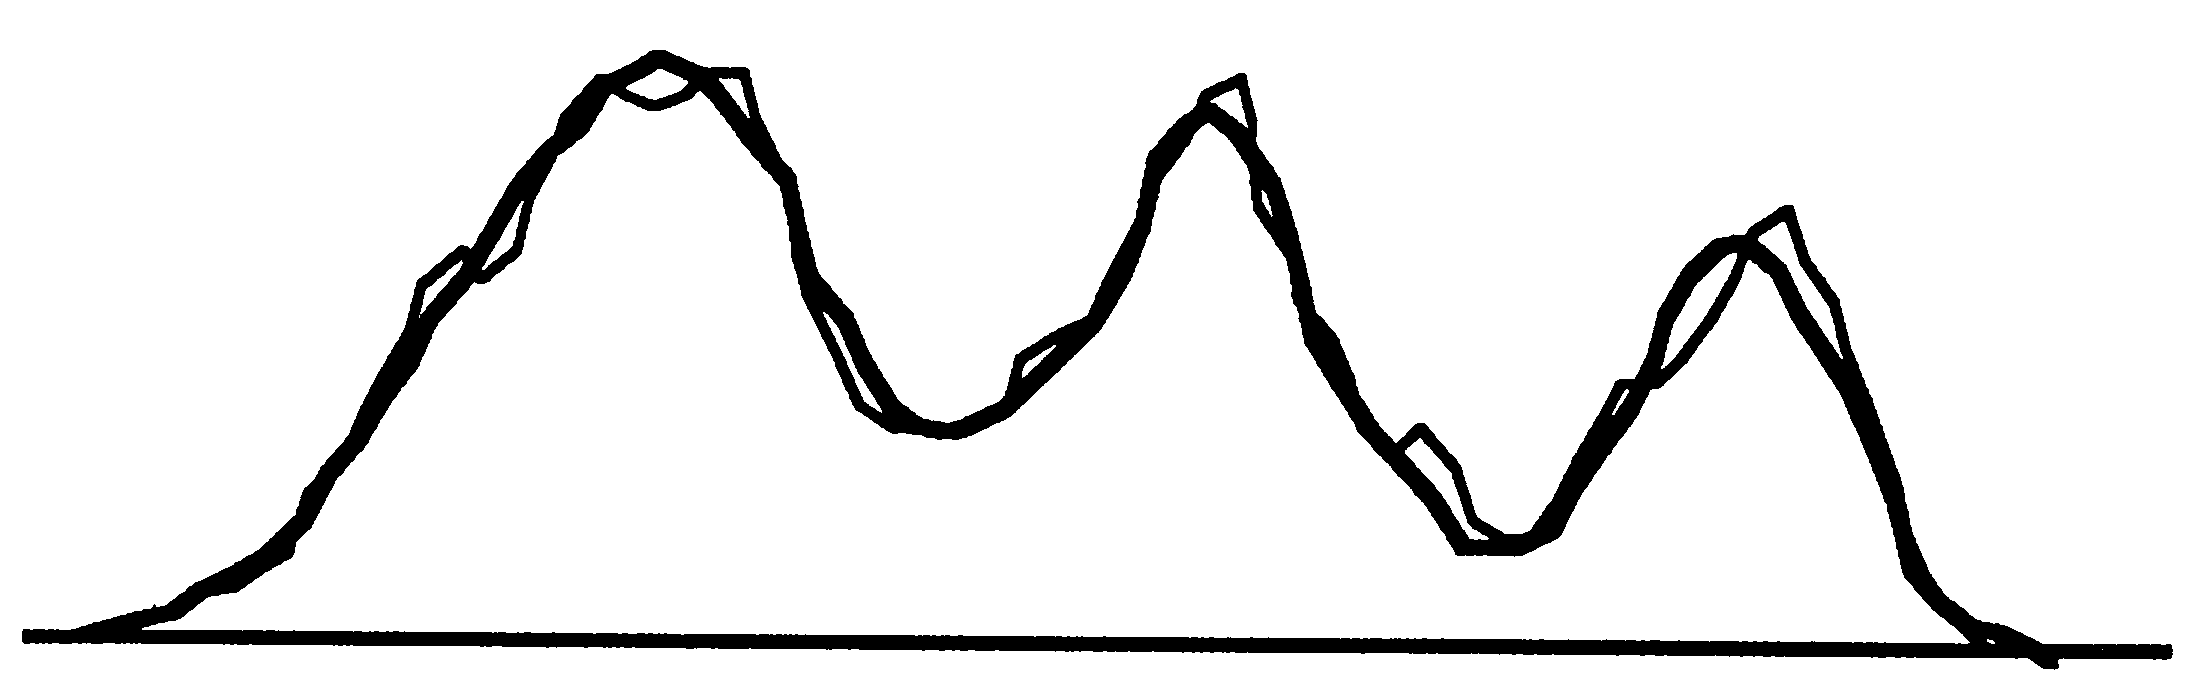
\includegraphics[scale=0.16]{figures/donoho.png}
    \caption{Thick line: A density with three modes. Thin line: The same density pertubed to have three modes. Taken from the paper of \textcite{Donoho1988-hg}.}
    \label{fig:donoho}
\end{figure}

The mean of normal model with known standard deviation is connected to three confidence intervals. The standard two-sided, the left-sided, and the right-sided. In this case, the two-sided confidence interval will always have finite diameter, or length, while the left-sided and right-sided will always have infinite diameter. But there are models and parameters where there is no confidence interval of guaranteed finite length. \textcite{Gleser1987-ii} proved a beautiful theorem giving sufficient conditions for there to be no confidence interval of guaranteed finite diameter. Essentially, if there is a sequence $\theta_n$ of parameters such that $|\theta_n| \to \infty$ while $f_{\theta_n} \to f$ for some density $f$, then there is no confidence interval for $\theta$ of guaranteed finite diameter. A simple example is $\theta = 1/\mu$, where $\mu$ is the mean of a normally distributed variable with fixed standard deviation. For in this case, $\mu_n = 1/n$ implies $\theta_n\to\infty$, while the density $f_\mu$ converges to a standard normal.
    \section{The replication crisis and meta-analysis}

In the 60s and 70s, there was a big conflict in clinical psychology. On one side were the Freudians, protective of the practice of psycho-dynamic therapy, a therapy based on concepts such as the unconscious and the importance of early life experiences. On the other side were the behaviourists, who mocked Freud's theory as unscientific, and preferred their variant of therapy, one that didn't need to postulate the existence of unobservables such as the unconscious \parencite[Chapter 4]{Wampold2019-fe}. It was against this backdrop the first meta-analysis was done. \textcite{Smith1977-vw} collected all available high-quality evidence on the efficacy of psychotherapies. They used statistical methods to integrate all of it into a whole. The main conclusions of this meta-analysis are still held to be true: 1.) Psychotherapy is an effective treatment and, 2.) there is no difference in effectiveness between different schools of therapy, the so-called \emph{Dodo bird verdict.}

The meta-analysis' competitor is the \emph{narrative review}, where the author uses her own expertise to amalgamate all the evidence she is aware of. The meta-analysis is preferred to a narrative review since it has a greater objectivity. A narrative review gives the author ample freedom to choose which studies to include, how to weigh the different studies, what questions or ideas to focus on and how to frame the results. In addition, a narrative review has no built-in safeguards against the biases of the author -- this allows for \emph{motivated reasoning} \parencite{Kunda1990-ry}, which could severely impact the quality of the review. On the other hand, a properly conducted meta-analysis allows for fewer of these choices. One reason for this is how meta-analysis deals with the protocols for collecting data and conducting analyses, as they should be registered beforehand \parencite{Egger1997-ue}; another is the transparency and replicability of the analysis. Meta-analyses does not allow idiosyncratic choices of how to frame problems, as statistical estimates are in focus. While a narrative review tells a story about a research field, a meta-analysis gives you dry, numerical quantities such as $\widehat{\mu}$ and $\widehat{s}$, quantities that should represent the most current, most objective estimates of the effect size and its standard error. The meta-analysis has been called the \emph{platinum standard of evidence}, playing on the claim that randomized controlled trials represent the gold standard of evidence \parencite{Stegenga2011-zo}.

But there is another, more practical reason to prefer meta-analyses over narrative reviews. When faced with studies numbering a hundred or more, it is a daunting task for any researcher to process the information in all of them without aid. The methods of meta-analysis allows the researcher to process such ``big data'' without suffering from information overload. Some data is especially difficulty to interpret and work with, for instance heterogeneous data, data with covariates, or the otherwise non-standard data. \parencite[][p. 2]{Borenstein2011-yx}

Since the primary results of a meta-analysis are statistics and $p$-values, the results can be interpreted in the same detached way as you would interpret individual studies. And the practical consequences of amalgamating evidence in this way can be dramatic. It can well be that all the published studies on a treatment are inconclusive, with effect sizes going in opposing directions and all $p$-values greater than $0.05$, but a meta-analysis of the exact same studies is definitive, demonstrating a positive effect without reasonable doubt. An example is the meta-analysis of \textcite{cannon_meta-analysis_2006} on the effect on heart attack prevention of high-dose statin therapy compared to standard-dose statin therapy. The meta-analysis covers four studies, where only one has a significant $p$-value. Still, the meta-analysis obtains a highly significant ($p<0.0001$) effect in the desired direction of better response to higher doses. 
\begin{figure}[h]
\noindent \begin{centering}
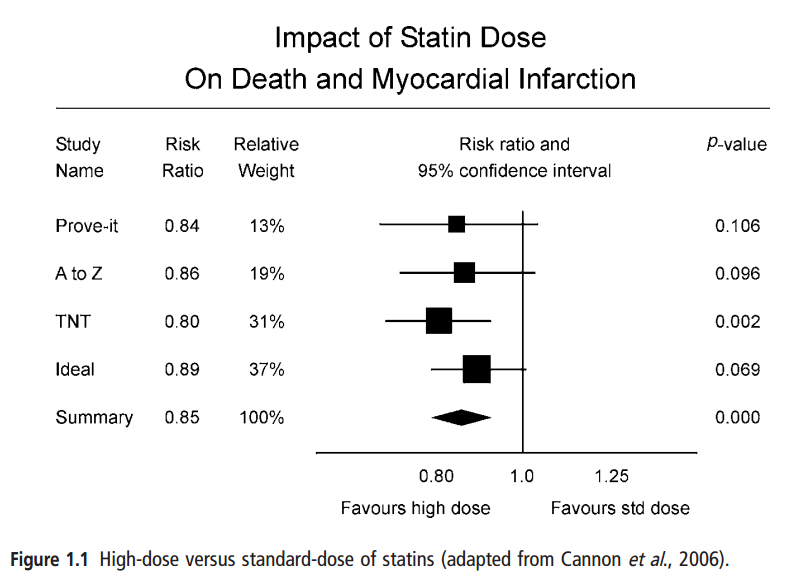
\includegraphics[scale=0.5]{figures/cannonetal2006}
\par\end{centering}
\caption{\label{fig:A-forest-plot}A \emph{forest plot} of the studies included
in \textcite{cannon_meta-analysis_2006} meta-analysis on statins. The
table is from \textcite[p. 4]{Borenstein2011-yx}.}
\end{figure}
Despite being terribly important, often the difference between life and death\footnote{See the preface of \textcite{Borenstein2011-yx} for a story of how earlier adoption of meta-analyses could have saved the lives of thousands of babies that suffered from sudden infant death syndrome.}, meta-analyses have two weaknesses. The first weakness is subjectivity. For while a meta-analysis is by nature less subjective than a narrative review, it might still be too subjective to settle a scientific question once and for all. This problem is emphasized by \textcite{Stegenga2011-zo}, and is exemplified by the continuing meta-analysis wars in the research on the effect of violent video games on aggressive behaviour, as discussed by \textcite{elson_twenty-five_2014}. The other weakness are systematic biases that are hard to model. One of these biases is \emph{publication
bias}, the tendency to publish only positive results. The other is
\emph{p}-hacking, the phenomenon where researchers unconsciously manipulate studies to get small \emph{p}-values.

\subsection{The problems of meta-analysis}
There is a certain degree of subjectivity in any data analysis, and the greater leeway to make subjective choices, the stronger the  tendency for the authors to make self-serving choices. An extreme variant of this is covered by \textcite{Steegen2016-fj}, where it was shown that a study about the combined effect of relationship status and fertility \parencite{Durante2013-yx} could be analysed in at least 210 different ways. Only some of these gave results in the desired direction and, not surprisingly, the published paper had results in the desired direction as well. 

The meta-analyst must choose which studies to include in her meta-analysis. There is often a good deal of subjectivity here, for it is rarely so that a study is unambiguously eligible for inclusion. There are many reasons to exclude a potential study from a meta-analysis. An oft-discussed bias is \emph{location bias}. If the meta-analysts are English, they will have a hard time incorporating foreign language studies into their meta-analysis \parencite{Egger1998-kj}, resulting in a location-specific meta-analysis. In addition, the meta-analyst will often include only studies from peer-reviewed scientific journals, ignoring studies from dissertations or the grey literature. There are trade-offs involved in the choice of including non-published studies. On one hand, inclusion of unpublished studies might reduce publication bias \parencite{Egger1997-ue}, but it could also increase the bias of the meta-analysis. The bias can increase since the meta-analyst must rely on her network of researchers to obtain the unpublished studies -- but her network is likely to be biased in exactly the same direction as she is. An example of this effect is found in \textcite{Ferguson2010-to}'s discussion of \textcite{Anderson2010-ki}'s meta-analysis on the effect of violent video games on behaviour. The literature on video game violence and aggression is divided into two camps. The camp associated with Anderson holds that violent video games cause aggression, the camp associated with Ferguson holds that they do not. In order for a meta-analysis to be accepted by all camps, it should not be biased against including studies from the opposite camp. However, \textcite{Anderson2010-ki} included several unpublished studies in their meta-analysis, but most were from their own Anderson's group or associated groups.
\begin{quote}
For example, of two unpublished studies, both are from Anderson et
al.'s broader research group. Of three in-press manuscripts
included, two (67\%) are from the Anderson et al. group. Of conference
presentations included, 9 of 12 (75\%) are from the Anderson et al.
group and colleagues. 
\begin{flushright}
-- \textcite[p. 2]{Ferguson2010-to}
\par\end{flushright}
\end{quote}
Another source of subjectivity is whether to only include randomized controlled trials. There is broad agreement that only randomized controlled trials should be included in a meta-analysis if these trials exists \parencite{Egger1997-ue}. The reason is that randomized controlled trials are not affected by confounders in the same way as e.g. case control studies and other observational studies. However, excluding observational studies violates the principle of total evidence, that your conclusions should be based on all available evidence, not just a subset of it, see \textcite{Stegenga2011-zo} for an extended discussion.

A reason to exclude a study is that it does not fulfil a list of best practices. Not all studies are created equal, some are simply of better quality than others. For instance, a subset of studies might have much better measuring instruments than the rest, making it reasonable to include only the studies with the good measuring instrument. But this is yet another source of subjectivity. As an example \parencite[][p. 6]{lakens_reproducibility_2016}, consider the following ``best-practice'' from \textcite{Anderson2010-ki}'s aforementioned meta-analysis on the effect of violent video games  on behaviour. In order to qualify for a best-practice study, the control group must be exposed to a non-violent game, while the treatment group must be exposed to a violent game. One unaccepted treatment-control pair was \emph{Mortal Kombat} vs \emph{Sonic the Hedgehog.} While Mortal Kombat is a fighting game infamous for its violence, Sonic the Hedgehog involves playing a hedgehog jumping on robots, and would easily be classified as among the least violent games by many researchers. On the other hand, an accepted treatment-control pair was \emph{Simpsons Hit \& Run} vs \emph{Grand Theft Auto 3}, even though Simpsons Hit \& Run involves pulling people out of their car in high-speed situations. 

Finally, studies can be excluded since they look suspicious. There are many cases of both reporting errors \parencite{Nuijten2016-eu} and downright fraud in the research literature, with Diedrik Stapel being a high-profile fraudster from social psychology. Since research data is seldom available, the meta-analyst will not be able to check the veracity of the reported results in each research paper. This can lead to exclusion of studies on seemingly ad-hoc grounds. As an example, take \citeauthor{ferguson_angry_2015}'s 2015 meta-analysis on the effect of violent video games on aggressive behaviour. In this analysis, he excluded the study of \textcite{gentile_effects_2009} due to what \textcite{ferguson_angry_2015} called ``bouncing beta'' regression coefficients, or regression coefficients of equal magnitude going in opposite directions, a choice heavily criticized \textcite{gentile_what_2015}.

\subsection{Publication bias and \textit{p}-hacking}

In 1959, \citeauthor{Sterling1959-cq} noted that many journals in psychology only regard an hypothesis as supported if its associated $p$-value was less than $0.05$. Then he hypothesized that this rigid rule would cause that studies with non-significant results not to be published. In order to test this hypothesis, he sampled $364$ papers from four psychology journals and registered the results from the statistical tests contained in them. The result was staggering: Out of $296$ significance tests, only $8$ were non-significant at the $0.05$ level. To account for such an observation without invoking publication bias would require extraordinary assumptions on the ability of psychologists to find real effects. The phenomenon that almost only publications with a $p$-value less than $0.05$ are published is commonly referred to as \emph{publication bias} or the \emph{file-drawer
problem} \parencite{rosenthal_file_1979}.

While the most famous cause of publication bias is the tendency for scientific journals to only accept articles containing statistically significant results, typically at the level of $0.05$ \parencite{simmons_false-positive_2011}, it should be understood more broadly, as the tendency to not publish null-results, or even weak results. The exact mechanism behind publication bias are unknown. For instance, a study reaching ``borderline statistical significance'' or even ``trending towards significance'', with a $p$-value at say $0.07$, is probably somewhat more likely to be published than a study with a $p$-value of $0.23$. If there is evidence for a null-effect, the paper is more likely to be published when the evidence for the null effect is strong, which is the case with large $n$ studies. Still, the cut-off at $p = 0.05$ is conspicuous. 

A cousin of publication bias is \emph{$p$-hacking}, the process of actively changing the data analysis in order to obtain significant results:
\begin{quote}
While collecting and analysing data, researchers have many decisions to make, including whether to collect more data, which outliers to exclude, which measure(s) to analyse, which covariates to use, and so on. If these decisions are not made in advance but rather are made as the data are being analysed, then researchers may make them in ways that self-servingly increase their odds of publishing. 
\begin{flushright}
-- \textcite[p. 1]{simonsohn_p-curve:_2014}
\par\end{flushright}
\end{quote}
As emphasized by \textcite{simonsohn_p-curve:_2014}, the presence of $p$-hacking creates bias even when \emph{all} conducted studies are published. In fields such as social psychology, where there is no consensus about how to measure different constructs, which statistical methods to use, or what variables your can condition on, it is almost always possible to get statistically significant result out of your study.\footnote{See \textcite[p. 2, study 2]{simmons_false-positive_2011} for a humorous instance of this, where a literally impossible phenomenon is established with $p<0.05$.} It is even possible to obtain enough results to fill four papers with spurious results, as was the case with food scientist Brian Wasnink \parencite{van_der_zee_statistical_2017}. This newfound focus on $p$-hacking changes how we view publication bias -- for instance, the common-sense claim that ``\emph{when a pattern is seen repeatedly in a field, the association is probably real, even if its exact extent can be debated}\textquotedblright{} (\textcite{ioannidis_why_2008}, cited in \textcite{simonsohn_p-curve:_2014}) is likely to be incorrect. Since $p$-hacking is commonplace, it is the popularity of a purported effect which determines the number of published studies on the same or similar effects, not the likelihood of obtaining a significant result.

Publication bias and \emph{p}-hacking are ubiquitous in psychology. A solid piece of evidence for this claim is the study of \textcite{Motyl2017-dx}. They collected all critical effect size estimates and \emph{p}-values from the four top-tier journals \emph{Journal of Personality and Social Psychology}, \emph{Personality and Social Psychology Bulletin}, \emph{Journal of Experimental Social Psychology}, and \emph{Psychological Science}. A critical effect size or \emph{p}-value is one that is used to support the core hypothesis of the paper. That is, the list of statistics does not include statistics associated with auxiliary questions such as ``are there significantly more woman than men in the sample''. These statistics were collected over the pre-replication crisis year
$2003$--$2004$ and the post-replication crisis years $2013$--$2014$. 

Figure \ref{fig:motyl} plots estimated effect sizes from \textcite{Motyl2017-dx} together with the line $y=1.96/\sqrt{n}$, the threshold for significance using the two-sided normal \emph{p}-value. The random effects meta-analysis model yields the estimates $\hat{\mu}_{0}=0.42$ and $\hat{\tau}_{0}=0.34$, Notice how the studies cluster just about threshold for significance, which would be extraordinarily unlikely under normal sampling.
\begin{figure}
\label{fig:motyl}
\noindent \begin{centering}
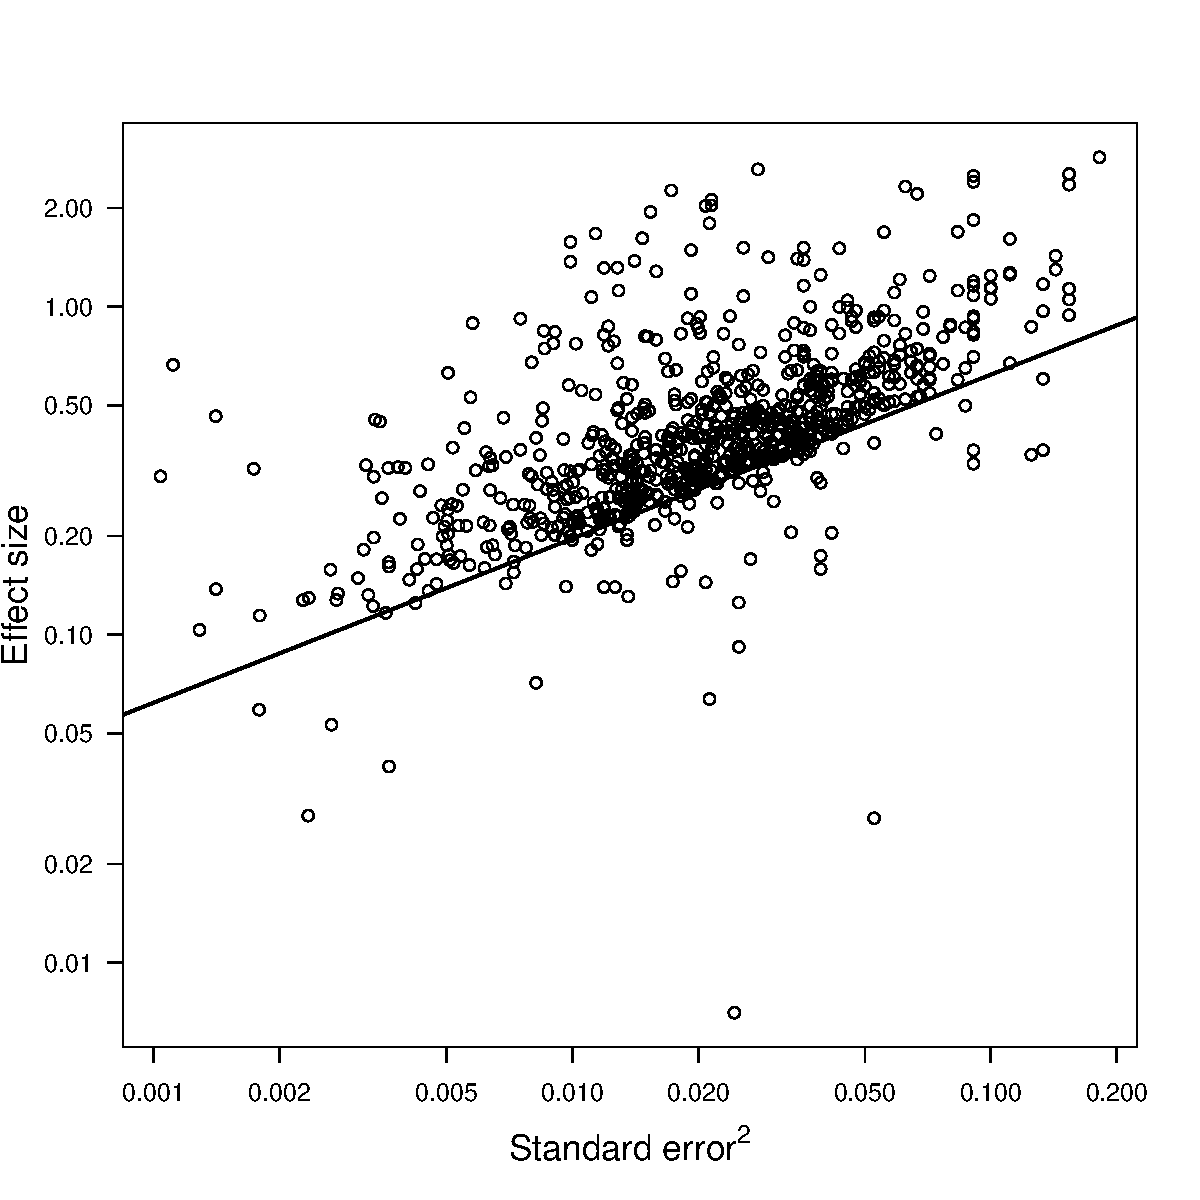
\includegraphics[scale=0.5]{figures/motyl}
\par\end{centering}
\caption{Estimated effect sizes and squared standard errors from \textcite{Motyl2017-dx}. The black line is $y=1.96/\sqrt{n}$, the threshold for significance using the two-sided normal \emph{p}-value. Both axes are logarithmic. The number of studies is $n=862$, and the percentage of significant results is $91.5\%$.}
\end{figure}
\subsection{Correction for publication bias and \textit{p}-hacking}

There are several methods that attempts to identify and even correct for publication bias. The most widely used is the \emph{funnel plot} of \textcite{Egger1998-kj}, where the standard error of each study is plotted against its effect size. Under severe publication bias, this plot will be skewed. This is because small studies, which will typically be those with high standard errors, must have large estimated effect sizes in order to cross the $p=0.05$ boundary. Figure \ref{fig:A-funnel-plot} contains an example of such a plot, based on a subset of the data in the video game and aggression meta-analysis of \textcite{Anderson2010-ki}, and made with the $\mathtt{R}$-package $\mathtt{metaphor}$. \parencite{viechtbauer_conducting_2010}.

\begin{figure}
\noindent \begin{centering}
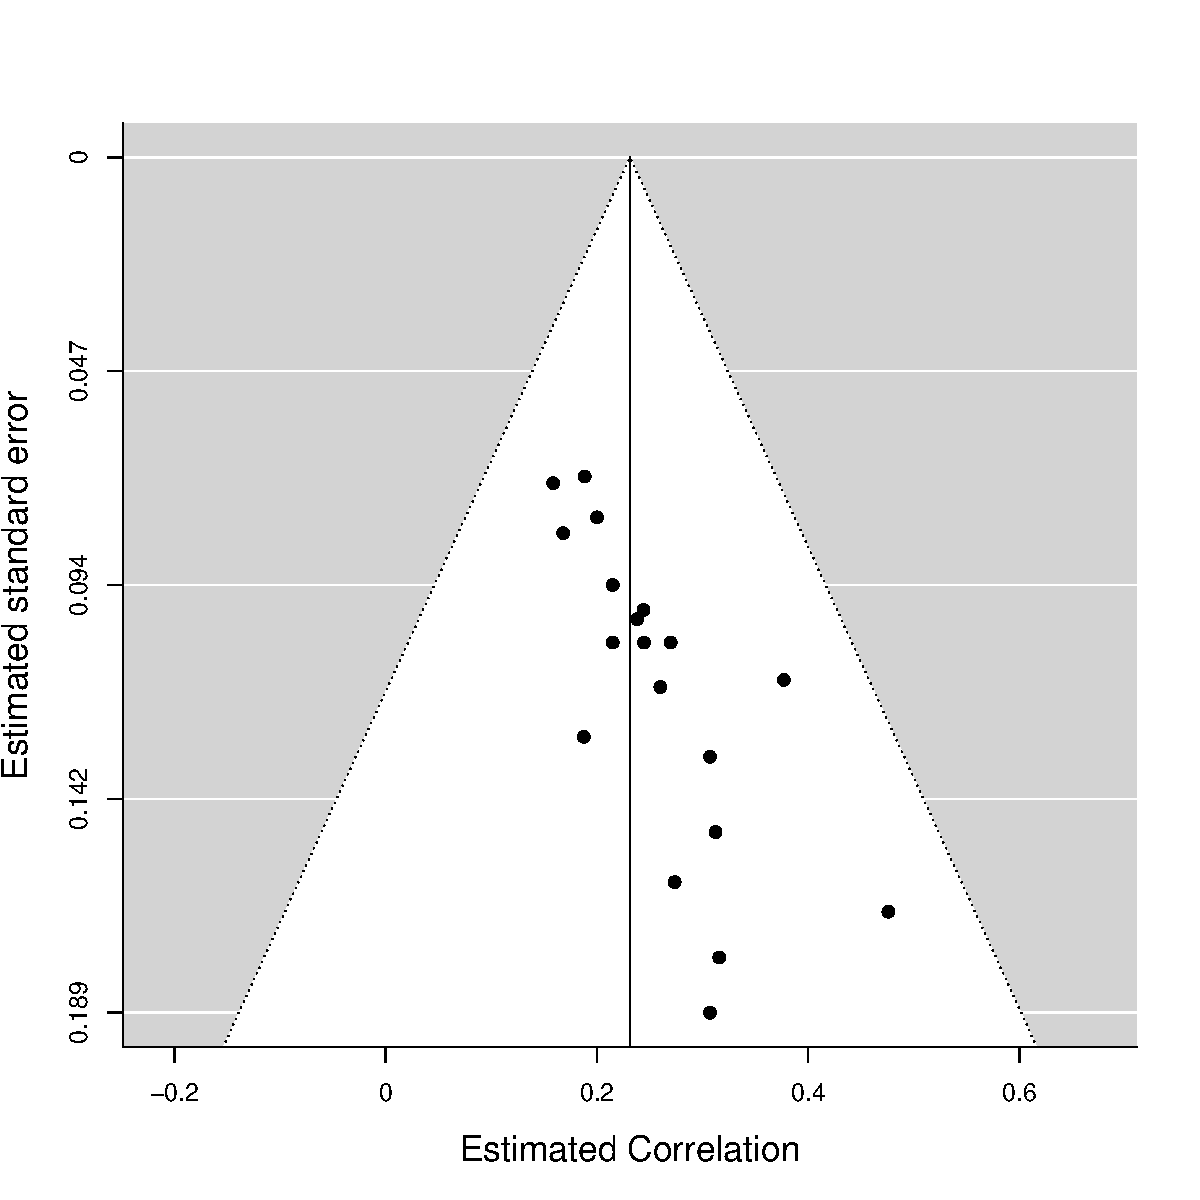
\includegraphics[scale=0.5]{figures/anderson}
\par\end{centering}
\caption{\label{fig:A-funnel-plot}A funnel plot of a subset from the meta-analysis of \textcite{Anderson2010-ki} on the effect of violent video games on aggressive behaviour. The funnel plot is highly skewed to the left, which indicates severe publication bias.}
\end{figure}

Taking inspiration from the funnel plot, \textcite{Egger1998-kj} propose to estimate a publication bias-corrected effect size by running the regression
\[
x_{i}\sim\theta+\beta\widehat{s}_{i}+\epsilon_{i},
\]
where $\theta$ is the adjusted effect size and $\beta\neq0$ indicates the presence of publication bias, a method called PET \parencite{stanley_beyond_2005}. But PET is not the only regression-based method for publication bias
correction. Another popular method is PET-PEESE \parencite{Stanley2014-gx}, a modified version of the above regression, applied mostly in economics research and more recently to psychology \parencite{carter_series_2015}. This method is not without critics. \textcite{gervais_putting_2015} claims the method systematically underestimates the effect size in presence of publication bias, making almost any effect appear to be indistinguishable from $0$. In addition, \textcite{simonsohn_[59]_2017} runs simulations to show that the method fails in presence of inter-study heterogeneity. The most popular method in medicine is named trim and fill \parencite{Duval2000-ct}, which is based on removing and adding non-observed studies to the funnel plot in order to make it symmetric. The $p$-curve of \textcite{simonsohn_p-curve:_2014} has proven to be popular in psychology. This method is based on the theoretical shape of the probability density function obtained from the $p$-values from a set of studies, under the null of no $p$-hacking,

The theoretically best justified model for publication bias are the selection models, which model publication bias directly using a rejection sampling method \textcite{Hedges1992-ue}. For a simulation study comparing methods to account for publication bias, see \textcite{moreno_assessment_2009} and \textcite{Carter2019-rw}.

All these methods, except the selection models, share a serious shortcoming. Popular statistical methods, such as linear regression and logistic regression, are based on explicitly defined models. These models allows for clear cut estimation of parameters, parameters with univocal definitions and interpretations. The methods for publication bias are not based on explicit models. As such, their estimated quantities are hard to interpret, and are defined in an offhand way. For instance, PET-PEESE is based on one half intuition, one half semi-rigorous mathematics; the $p$-curve of is based on statistical properties of a null-model we assume that is false. 

The meta-analyst will have to choose whether to correct for publication bias or not. If she opts to correct for publication bias, she is faced with a large number of different methods, most of them not particularly good. But if her choice is no, her resulting estimates might be severely biased. The effect of this choice is potentially tremendous. As an illustration, take a well-known contentious issue from economics: what is the relationship between the minimum wage and employment? The predictions from economic theory about this are unequivocal. Rising the minimum wage should raise the rate of unemployment. There are two reasons why: First, when the minimum wage is raised above the competitive wage, the employer will shift his spending towards other venues such as capital investments. Second, the industries affected will increase their prices to consumers, reducing the demand for labour in turn. \textcite{doucouliagos_publication_2009} studies the empirical research on the relationship between a minimum wage floor and employment. Their meta-analysis contains $64$ studies, which in turn contain a total of $1474$ employment elasticity estimates. The average elasticity was $-0.19$, while the fixed effects meta-analytic estimate was $-0.054$, both highly significant. However, their publication bias-corrected estimate was the meagre $-0.01$. In the words of \textcite{doucouliagos_publication_2009}: ``An elasticity of -0.01 has no meaningful policy implications. If correct, the minimum wage could be doubled and cause only a 1 per cent decrease in teenage employment.'' In this case the decision to correct for publication bias reduced the effect size estimate with a factor of $5$. Needless to say, this could have huge policy implication, considering the recent push towards rising the minimum wage in California and other U.S. states \parencite{Lee2016-bd}.

Since publication bias and $p$-hacking are everywhere and their effect can make the difference between two radically different conclusions, good methods for dealing with them are needed. Even more important, scientists should be rigorous in their usage of methods designed to avoid publication bias and $p$-hacking, for instance study pre-registration. Most importantly, science should be open, transparent, and reproducible. 

\subsection{Open science}
\label{subsec:open science}
Scientific data is hard to get by request, even for editors. In an editorial for the neuroscience journal Molecular Brain, \textcite{Miyakawa2020-ze} described his experience with asking authors for raw data. Out of the $180$ submissions he handled, he made $41$ requests for raw data as part of a ``Revise before review'' decision. Among these $41$ manuscripts, $21$ withdrew their submission. Out of the $20$ manuscripts left, Miyakawa rejected $19$ due to insufficient raw data. Thus $97\%$ of the submissions failed to provide raw data of good quality even after a request. Miyakawa suggests the possibility ``that the raw data did not exist from the beginning, at least in some portions of these cases.''

Data is even harder to get for non-editors. As part of a study of psychological research's robustness to outliers, \textcite{Wicherts2006-yy} requested data from $141$ research psychologists, but received some data from only $27\%$ percent of them. This was not plausibly because the data was lost: all of the papers they requested data from were published during the last $12$ months. Moreover, the contacted psychologists reneged on their duty. All of them had signed the American Psychological Association's $2001$ ethics code, which contains the sentence ``psychologists do not withhold the data on which their conclusions are based from other competent professionals'' \parencite[p. 396; as cited in Wicherts et al. 2006][]{American_Psychological_Association2001-rs}. 
\textcite{Wicherts2006-yy} are not the only researchers who have had trouble getting data. \textcite[p. 526]{Nelson2018-ov} wrote: 
\begin{quote} Requesting data from another researcher---particularly for the stated justification of suspecting fraud---is socially taxing. Furthermore, although the APA prescribes the sharing of data, there is no enforcement mechanism. We have heard many stories from other researchers who were told that the requested data were coming soon (but then never arrive), were impossible to share, had been lost, or were legally impounded. We have personally been denied data explicitly because the authors wished to avoid criticism; the authors wrote bluntly, \textquotedblleft no data for you.''
\end{quote}
There are some valid reasons not to share data. Most important is the issue of privacy, where there are both ethical and legal issues. But for the majority of psychology papers, the reasons for not sharing data are bad. It is natural to suspect that data is withheld since the authors want to avoid criticism or scrutiny, and there is some evidence for this suspicion. Using the data from the aforementioned study of \textcite{Wicherts2006-yy}, \textcite{Wicherts2011-eb} argue that the reluctance to share data is associated with the study's quality. For instance, $25\%$ of the studies that did not share data reported \textit{p}-values below $0.05$ when they were not, in fact, below $0.05$; this error was not committed by any of the studies that shared data.

The benefits of sharing data are numerous, and not always obvious. \textcite{Wicherts2012-cp} lists six points. First, sharing data preserves it. If you keep your data only on your own computer, it will eventually be lost. Second, openness allows other researchers to independently reproduce your results. They can uncover errors in the analysis, \emph{p-}hacking, or scientific misconduct. Third, publishing data can make the paper more citable. This is especially relatable for methodologists, who frequently cite papers only since they are associated with data sets. Fourth and fifth, other researchers can run different analysis on your data. For statisticians this one is an obvious one, and is especially important for meta-analysists \parencite{Cooper2009-ge}. Finally, founding agencies routinely stipulate that data must kept in an accessible form for some minimum amount of years. If the data are made open, you do not have to worry at all about this.  

A major reason to demand open data is to prevent scientific fraud. While most researchers believe that fraud is uncommon, measuring it is arduous. Since there are strong incentives to falsify data and incorrectly report summary statistics, it is imprudent to assume no one does it. Demanding open data reduces the number of fraudulent papers by two mechanism. First, you are strongly disincentivized to falsify data and summary statistics when the data are publicly available. For other researchers can, in principle, uncover your fraud at any moment. Second, fraudulent papers will be uncovered at a greater rate when the evidence is available for scrutiny. 

By merely looking at reported standard deviations and means, \textcite{Simonsohn2013-ul} started to suspect two authors of systematic data manipulation. Luckily, the authors supplied him with the raw data, which only strengthened the suspicion of fraud. One of the authors, Dirk Smeesters, has now been convicted of scientific misconduct. The other, Lawrence Sanna, suddenly resigned from his professorship. However, \textcite{Simonsohn2013-ul}
also observed a ``third case of exceedingly similar summary statistics''. Sadly, he did not get hold of the data, as the ``main author reported losing them, and the coauthors of the article did not wish to get involved''.

Papers report inconsistent statistics. \textcite{Nuijten2016-eu} reports that one of two psychology papers contains \emph{p}-values that are inconsistent with its reported test statistics. Moreover, one of eight papers have gross inconsistencies, where a reported \emph{p}-value is significant but its computed \emph{p}-value is not. As a reader without access to either the data or the code used to calculate the statistics, you are left in the dark about what the data actually says.

\textcite{John2012-xp} measured the frequency of \emph{p}-hacking and other questionable research practices in psychology using an electronic survey. Figure \ref{fig:john2012} shows their results. Most of these questions are about \emph{p}-hacking, but question eight is about \emph{hypothesising after results are known} (denoted \emph{HARKing} by \textcite{Kerr1998-by}), and question ten is about scientific fraud. Approximately one third of the respondents admitted to hypothesising after results are known. Doing this certainly makes \emph{p}-values invalid, as choosing a null hypothesis conditioned its \emph{p}-value being less than $0.05$ definitely makes you reject the null hypothesis. But hypothesising after results are known is detrimental for other reasons too, see \textcite[p. 205]{Kerr1998-by} for nine more reasons why.

\begin{figure}
\noindent \begin{centering}
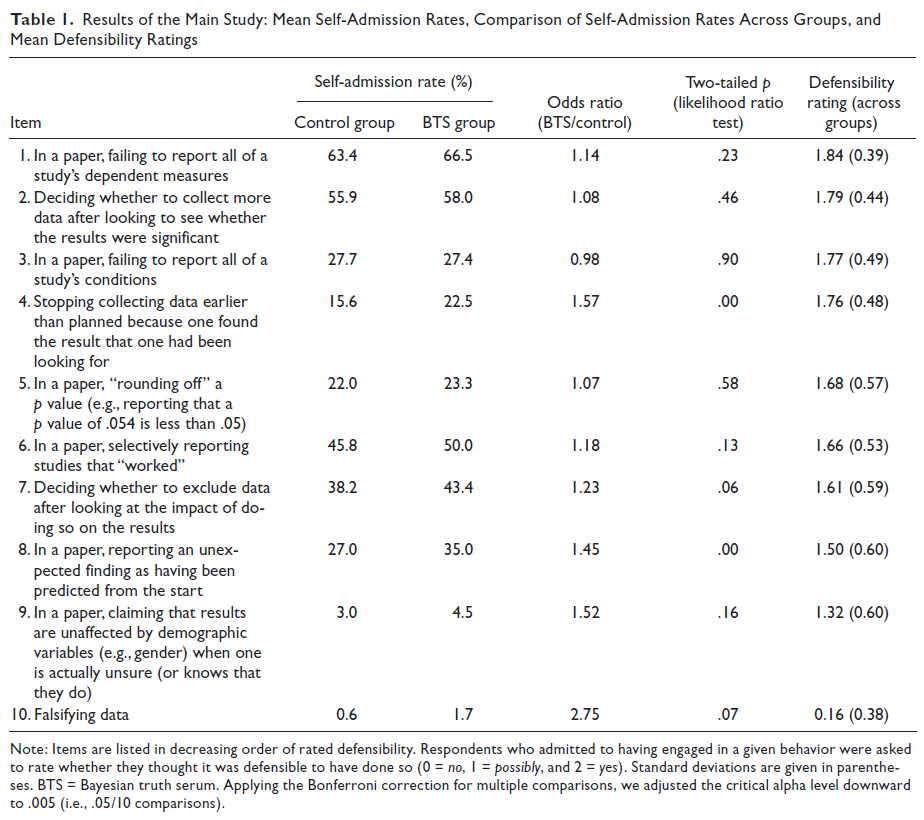
\includegraphics[scale=0.4]{figures/john2012}
\par\end{centering}
\caption{\label{fig:john2012}Self-admission rates to questionable research practices from \textcite{John2012-xp}. The participants in the BTS group were given incentives for honest reporting, and the defensibility rating indicates how defensible the respondents consider each practice to be.}
\end{figure}

A study is preregistered if it is planned in detail in advance and this plan is publicly known \parencite{Van_t_Veer2016-fo}. The plan should specify which hypotheses are tested, the experimental methods used, and the statistical analysis exactly. A benefit of proper preregistration is that it makes hypothesising after results are known impossible, which on its own should reduce the rate of false positives in the literature quite a bit. But preregistration is also a remedy for \emph{p}-hacking, and can even help with publication bias.

\textcite{Scheel2020-sq} studied rate of positive results in standard research versus preregistered research. Among $148$ standard, non-preregistered studies sampled, $142$ were positive. That is, $95\%$ were positive. On the other hand only $15/30=50\%$ of the preregistered reports were positive. Such a rate of positive results is far more plausible than $95\%$, especially when seen in light of the fact that most psychological research is severely underpowered \parencite{Sedlmeier1989-zz}.

% \subsection{Back-of-the-envelope calculations }
% A large part the daily lives of researchers is spent on reading and critically engaging with other peoples research. Prior to the replication crisis, a common way to judge the worth of an effect was to look at its \emph{p}-value or \emph{t-}value. If the \emph{p}-value was smaller than $0.05$, or the \emph{t-}value larger than approximately $2$, results looked impressive enough to be worthy of consideration. While plenty of researchers believe this way to consume research is bad \parencite{Gigerenzer2004-oc}, it is not without its merits. We have limited attention spans and need to abide by some decision rules; what we need are well-justified decision rules that will not lead us astray with an unacceptably high probability.

% Making a couple of half-plausible assumptions, there are some simple ways to correct isolated studies for publication bias and \emph{p}-hacking. We will take a short look at two back-of-the-envelope methods, one for expectations and one for effect sizes. Both are based on a simple model of selection for significance, where we observe only significant normal $X$s. Assume $X\sim N(\mu,n^{-1/2})$ and let $U=\Phi(-n^{1/2}X)$ be the standard one-sided $p$-value. 

% Let's have a look at the corrected expectation first. The expectation of the left-truncated normal is \parencite[Section 10.1]{Johnson1994-ag}
% \begin{equation}
% \mu+\sigma M'\left(\frac{a-\mu}{\sigma}\right),\label{eq:mean of truncated normal}
% \end{equation}
% where
% $M'(\text{\ensuremath{\theta}})=\phi(\text{\ensuremath{\theta}})/\Phi(-\text{\ensuremath{\theta}})$
% is the inverse Mills' ratio. 
% In our case, $a=c_{\alpha}n^{-1/2}$ and $\sigma=n^{-1/2},$ and the expectation equals $\mu+n^{-1/2}M'(c_{\alpha}-n^{1/2}\mu)$, where $c_\alpha = \Phi^{-1}(1-\alpha)$. When
% $\mu=0$ and $\alpha=0.05$, we get $E(X\mid n^{1/2}X>c_{\alpha})=n^{-1/2}\alpha^{-1}\phi(c_{\alpha})\approx2n^{-1/2}.$
% This value is easy to remember and compute, and provides a realistic baseline to compare effect sizes against. In a world free of biases, we would informally compare an effect size against $0$. In a world with publication bias and \emph{p}-hacking, comparing against $2n^{-1/2}$ is smarter and almost as easy. From the data set of \textcite{Motyl2017-dx} we just looked at, we get $2\overline{n^{-1/2}}=0.24$. That is, we would expect a mean effect size of $0.24$ from psychology even when the true mean is $0$, assuming complete selection for significance and the validity of the normal approximation. The actual mean of the data set, $\overline{\theta}=0.45$, does not look that impressive any more.

% There are strong reasons not to care only about \emph{p}-values, but also about effect sizes \parencite{Funder2019-tg}. The natural way to
% estimate the effect size $\mu$ is to use the maximum likelihood estimator $\hat{\mu}$. While this quantity is easy to calculate numerically, it is hardly convenient to use when reading a paper. Luckily, there are simple bounds for the maximum likelihood estimator.
% \begin{proposition}
% \label{prop:maximum likelihood bounds}The maximum likelihood estimator of $d$, called $\hat{d}$, based on a single observation $x$ from a study with $n$ participants is bounded by 
% \[
% l(x)\leq\hat{d}(x)\leq u(x).
% \]
% The bounds are equal to
% \begin{eqnarray}
% l(x) & = & x-\frac{1}{n^{1/2}\delta},\label{eq:lower bound}\\
% u(x) & = & x-\frac{1}{n^{1/2}\delta}\max\{1-\delta^{2},0\}.\label{eq:upper bound}
% \end{eqnarray}
% where $\delta=n^{1/2}x-\Phi^{-1}(1-\alpha)$.
% \end{proposition}

% You could argue that $\delta$ does not look that simple to work with, but it is. For $n^{1/2}x$ is the \textit{t}-value, which is often reported in the paper itself. The value of $\Phi^{-1}(1-\alpha)$, on the other hand, equals $1.96$. It might be profitable to increase it slightly, to e.g. $2$, to account for the fact that \textit{t}-tests are frequently used. Now $n^{1/2} - \Phi^{-1}(1-\alpha) \approx t - 2$, which is easy to calculate by hand. If $1/(t - 2)$ value is too big compared with $n^{1/2}$, you can probably disregard the study. 

% Consider Study 1 of the infamous \emph{power posing} paper by \textcite{Carney2010-we}. Here $t = 2.07$, so that $1/(t - 2) \approx 14$ with $38$ degrees of freedom. Since $38^{1/2} \approx 6$, we see that $1/(t - 2)$ is much larger than $38^{1/2}$, and we can probably ignore the study.

% Proposition \ref{prop:maximum likelihood bounds} is a straight-forward
% corollary of the following proposition. 
% \begin{proposition}
% \label{prop:ml bouds}Let $X_{1},\ldots,X_{N}$ be independent samples
% from a left-truncated normal. Assuming known truncation point $a$
% and standard deviation $\sigma$, the maximum likelihood estimator
% $\hat{\mu}$ of $\mu$ is bounded by
% \begin{equation}
% \overline{x}-\frac{\sigma^{2}}{\overline{x}-a}<\hat{\mu}<\overline{x}-\max\left(\frac{\sigma^{2}}{\overline{x}-a}-(\overline{x}-a),0\right).\label{eq:ml bounds}
% \end{equation}
% \end{proposition}
% \begin{proof}
% Differentiating the logarithm of the density of a truncated normal,
% we find that the maximum likelihood estimator is the solution to $\mu=\overline{x}-\sigma M'([a-\mu]/\sigma)$. The inverse Mills' ratio can be bounded
% elementary functions \parencite{Yang2015-pa}. In particular, it can be
% bounded by \parencite[Equation 32]{Gasull2014-hn}
% \begin{equation}
% M_{u}(\theta)=\frac{1}{2}(\sqrt{\text{\ensuremath{\theta}}^{2}+4}+\text{\ensuremath{\theta}})>M'(\text{\ensuremath{\theta}}),\label{eq:Mills' ratio inequality}
% \end{equation}
% and 
% \begin{equation}
% M'(\text{\ensuremath{\theta}})>\frac{1}{4}(\sqrt{\text{\ensuremath{\theta}}^{2}+8}+3\text{\ensuremath{\theta}})=M_{l}(\theta)>\theta.\label{eq:Mill's ratio inequality (2)}
% \end{equation}
% The functions $M(\text{\ensuremath{\theta}})$ in these inequalities
% are increasing in $\text{\ensuremath{\theta}}$, hence $\overline{x}-\sigma M([a-\mu]/\sigma)$
% is increasing in $\mu$. Assume $\mu_{u}$ satisfies $\mu_{u}=\overline{x}-\sigma M_{u}([a-\mu_{u}]/\sigma)$.
% Since $M_{u}(\theta)>M'(\theta)$, we have $\overline{x}-\sigma M'([a-\mu_{u}]/\sigma)<0$
% too, thus $\mu_{u}<\hat{\mu}$. Likewise, if $\mu_{l}$ satisfies
% $\mu_{l}=\overline{x}-\sigma M_{l}([a-\mu_{l}]/\sigma)$, then $\mu_{l}>\hat{\mu}$.
% Now define $l(\overline{x})=\mu_{u}$ and $u(\overline{x})=\mu_{l}$.
% Now, to find $l(\overline{x})$, solve
% \[
% \mu=\overline{x}-\sigma\frac{1}{2}\left(\sqrt{\text{\ensuremath{([a-\mu]/\sigma)}}^{2}+4}+\text{\ensuremath{[a-\mu]/\sigma}}\right)
% \]
% to get $\mu=\overline{x}-\sigma^{2}/(\overline{x}-a)$. The upper
% bound $u(\overline{x})$ can be found in the same manner, using both
% the lower bounds $M_{l}(\theta)$ and $\theta$ and choosing the best
% option.
% \end{proof}
    
\section{Psychometrics}
In the animated 1937 classic \textit{Clock Cleaners}, Mickey Mouse, Donald Duck, and Goofy are working as janitors in a clock tower. As usual, Goofy is dimwitted and carefree, Donald Duck gets fits of anger, and Mickey Mouse is kind and compassionate. Goofy mistakes a statue for a lady, Donald Duck throws a temper tantrum at a spring, and Mickey Mouse does everything he can to save Goofy from falling to certain death. This is not the only animated movie were these characters behave like this. Donald Duck's fiery temper -- and bad luck -- is what he's known for, and something you'd expect to see in any movie featuring him. Likewise, Goofy is always thickheaded. We say that these characters have \textit{stable psychological traits}. And real humans have them too. There are people you would describe as temperamental. In almost every situation, they are more prone to getting angry than others.

Psychometrics is about the study and quantification of psychological traits such as temperament. These traits cannot be directly measured though. Even if you think every individual has, in Platonic sense, a real variable $Z$ called "temperament", you would not be able to measure it directly. For these traits are not observable, they are \textit{latent}. Instead of observing $Z$ directly, we observe a random vector $X$ of proxies for $Z$. In most cases these proxies are responses to a questionnaire, usually on \emph{Likert items}. A Likert item is the response to a question with ordered alternatives ranging from e.g. strongly disagree to strongly agree. Table \ref{tab:IPIP} shows five questions from the International Personality Item Pool \parencite{Goldberg1992-hp}, all of them supposedly related to the trait \textit{agreeableness}.

\begin{table}
\caption{\label{tab:IPIP}Five questions loading on \textit{agreeableness} from the International Personality Item Pool}
\noindent \begin{centering}
\begin{tabular}{lccccc}
 & $1$ & $2$ & $3$ & $4$ & $5$\tabularnewline
Am indifferent to the feelings of others.  & $\bigcirc$ & $\bigcirc$ & $\bigcirc$ & $\bigcirc$ & $\bigcirc$\tabularnewline
Inquire about others' well-being. & $\bigcirc$ & $\bigcirc$ & $\bigcirc$ & $\bigcirc$ & $\bigcirc$\tabularnewline
Know how to comfort others. & $\bigcirc$ & $\bigcirc$ & $\bigcirc$ & $\bigcirc$ & $\bigcirc$\tabularnewline
Love children. & $\bigcirc$ & $\bigcirc$ & $\bigcirc$ & $\bigcirc$ & $\bigcirc$\tabularnewline
Make people feel at ease.  & $\bigcirc$ & $\bigcirc$ & $\bigcirc$ & $\bigcirc$ & $\bigcirc$\tabularnewline
\end{tabular}
\par\end{centering}
\vskip7.0pt
\noindent \centering{}{\scriptsize{}1, Very Inaccurate; 2, Moderately
Inaccurate; 3, Neither Accurate Nor Inaccurate; 4, Moderately Accurate;
5, Very Accurate}{\scriptsize\par}
\end{table}

These questions are said to \textit{load on} the personality trait agreeableness. A person strongly agreeing with ``Am indifferent to the feelings of others.'' is likely to be disagreeable, and his affirmative answer is likely to be caused by his disagreeableness. Psychometrics is about using questions such as these to infer, numerically, how agreeable someone is. That is, the questions serves as proxies for the latent variable, and it is the latent variable we are actually interested in. The answers to the individual questions are not too interesting in and of themselves.

To be able to connect proxies to their latent variables, will need a statistical model. The most popular model is the linear model. Here $Y$ is a $J$-ary vector and
\begin{equation}
Y=\lambda Z+\Psi^{1/2}\epsilon,\label{eq:one-factor model}
\end{equation}
where $\Lambda$ is a real matrix of \emph{factor loadings}, $\Psi$ is a positive definite matrix, $\epsilon$ is a $J$-ary vector of uncorrelated error terms, and both $Z$ and $\epsilon$ have finite variances. This is the linear factor model. Of particular interest is the \textit{one-factor model}, where $Z$ is scalar and $\Lambda = \lambda$ a vector of loadings.

The linear factor model is a member of the wider class of generalized item response models \parencite{Mellenbergh1994-iy}, which encompasses most psychometric models \parencite[Chapter 3.1]{Borsboom2005-iq}. A generalized item response model is similar to a generalized linear model. Let $X$ be a vector of covariates, $Z$ be a vector of latent variables, $g$ a monotone link function, and $Y$ the $J$-ary vector of responses. Then 
\begin{equation}
g(E[Y_{j}])=\lambda_{j}^{T}Z+\beta_{j}^{T}X,\quad(j=1,\ldots J)\label{eq:GLIRT model}
\end{equation}
is a generalized item response model.

The most important feature of psychometric models is the reversed roles of regressors and covariates. In a usual regression model, the left hand side is unknown and the input to the right hand side is known. For instance, when we regress gross domestic product on some other economic indicators, we wish to predict gross domestic product from those other indicators. We can imagine a situation where we know the economic indicators and make a guess about gross domestic product. 

In psychometrics this situation is turned on its head. We know the regressors but not all of the covariates. In the words of \textcite[p. 61]{Borsboom2005-iq}, models in psychometrics are \emph{reflective}, not \emph{formative}. In a formative model, and variable $Y$ is defined in terms of its indicator. For instance, socio-economic status is defined in terms of variables such as income, education level, and neighborhood quality. But socio-economic status does not cause them, it is merely a summary \parencite[p. 62]{Borsboom2005-iq}. On the other hand, agreeableness causes the responses to the questions in Table \ref{tab:IPIP}. Figure \ref{fig:dag} shows formative and reflexive models using directed graphs, where directed arrows are interpreted causally.

\begin{figure}
\noindent \begin{centering}
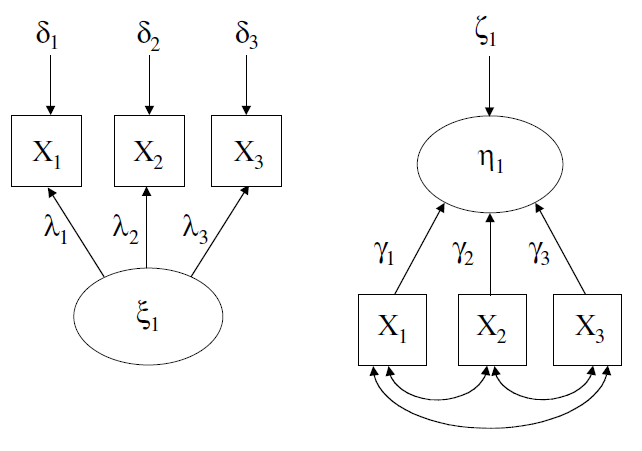
\includegraphics[scale=0.5]{chunks/borsboom}
\par\end{centering}

\caption{\label{fig:dag}(left) A reflexive model where the latent variable $\xi_{1}$ causes the observed $X_{i}$s. (right) A formative model where $\eta_{1}$ is defined in terms of the $X_{i}$s. This figure is taken from \textcite[p. 61]{Borsboom2005-iq}.}
\end{figure}

When we have a psychometric model such as the one-factor model, we want to estimate the latent $Z$. Disregarding potential covariates $X$, an estimator of $Z$ must be based on the vector of observed variables $Y$ only. That is, $\hat{Z}=\phi(Y)$, a function of the observed variables $Y$. For generalized item response models, the maximum likelihood estimator of $Z$ or its posterior mean are common estimators of $Z$. These quantities are only defined when we make parametric assumptions about all random variables involved. But the linear one-factor model is a semi-parametric model, and the maximum likelihood estimator of $Z$ need not exists. The most widely used estimator of $Z$ in psychology is the \emph{sum
score}, $\hat{Z}=\sum_{i=1}^{k}Y_{i}$, and the mean squared error-optimal linear combination $\hat{Z}=\sum_{i=1}^{k}v_{i}Y_{i}$ is popular too. Both of these make sense mainly in the linear one-factor model. 

The three fundamental questions of psychometrics are:
\begin{enumerate}
\item \textbf{Model fit}. Is the model a good approximation to reality? Are the structural and parametric assumptions defensible? Model fit in structural equation modelling is usually evaluation through model fit indices, for instance $\chi^{2}$-tests. \parencite[Chapter 15]{Mulaik2009-gc}.
\item \textbf{Reliability}. Is $\hat{Z}$ a good estimator of $Z$, assuming the model is correct? If so, the estimator is reliable. In the linear one-factor model, the reliability is most often measured by calculating coefficient alpha \parencite{Cronbach1951-in}, a statistic related to the squared correlation $\Cor^{2}(Z,\hat{Z})$. between $Z$ and $\hat{Z}$ when $\hat{Z}$ is a sum-score.
\item \textbf{Validity}. Is $Z$ what we want it to be? Even if the model is correct, $Z$ might be something else than what we would like it to be. For instance, the five questions of Table \ref{tab:IPIP} should be related to the personality trait agreeableness. But is true? Maybe they measure some other psychological trait, such as irritability, intelligence, or even a physical trait such as height. Assuming personality traits such agreeableness exists, which not every psychometrician agrees with, there are some methods to check this. The techniques are often extrastatistical, and the application of them is called \emph{validation}. \parencite[Chapter 6]{Borsboom2005-iq}
\end{enumerate}

\subsection{Reliability}

There is a mismatch between the mathematical definition of reliability and what psychologists think reliability is. The common definition of reliability is slightly different from correlation-based definition above. In our terminology, \textcite[Equation 3]{Raykov2019-yr} defines the reliability of $\hat{Z}$ as a measurement of $Z$ as
\begin{equation}
\rho=\frac{\Var Z}{\Var\hat{Z}}\label{eq:rakov-reliabiliy}
\end{equation} Under the linear model \eqref{eq:one-factor model}, $\rho = \Cor^2(Z,\hat{Z})$ when $Z$ is a linear predictor of $Z$ with zero mean, which happens when $Z$ is the sum-score $\hat{Z}=\sum_{i=1}^{k}Y_{i}$ or the mean squared error-optimal linear combination $\hat{Z}=\sum_{i=1}^{k}v_{i}Y_{i}$.

Both the correlation and ratio of variance definitions of reliability are straight-forward. Both are defined relative to statistical model, and both inform us about the quality of $\hat{Z}$ as a predictor of $Z$. But it is common for psychologists to hope for much more. For instance, \textcite{McNeish2018-vu} wrote that
\begin{quote} 
[...] researchers often report a measure of reliability to demonstrate that the items composing the measure are reliable, meaning that the scores based on the items are reasonably consistent, the responses to the scale are reproducible, and that responses are not simply comprised of random noise. Put another way, a reliability analysis provides evidence that the scale is consistently measuring the same thing [...]
\end{quote}

It is hard to reconcile all these claims with the definition of reliability, except that the responses cannot be random noise only. The claim that reliability analyses provide evidence that the scale consistently measure the same thing makes some researchers call reliability coefficients measures of internal consistency. This notion is incorrect, as the reliability coefficient cannot be used to differentiate between factors model with one or more factors \parencite[]{McDonald1981-xz}.

I do not claim that reliability coefficients are useless. If you have reason to believe in your model, a high reliability coefficient is nice to have, as it allows you to predict $Z$ well. But just as $R^2$, it is not a measure of model fit \parencite{Helland1987-eb}. Just as the $R^2$ can be small even if the linear model fits exactly, the reliability coefficient can be small even when the responses to the scale are reproducible and the scale measures the same thing. 

Reliability coefficients are ubiquitous in psychology. The most used coefficient is coefficient alpha, also known as Cronbach's alpha. This coefficient is the reliability for the sum-score under the linear one-factor model \eqref{eq:one-factor model} assuming $\tau$-equivalence, i.e., $\lambda_i = \lambda_j$ for all $i,j$. Its definition is 
\begin{equation}
\hat{\alpha}=\frac{k}{k-1}\left(1-\frac{\tr{S}}{\boldsymbol{1}^{T}S\boldsymbol{1}}\right),\label{eq:sample coefficient alpha}
\end{equation}
where $k$ is the size of $Y$, the vector $\boldsymbol{1}$ is a $k$-ary vector of only ones, and $S$ is the covariance matrix of $Y$. It is straight-forward algebra to verify that coefficient alpha equals the reliability for the sum-score $\hat{Z}$ under the $\tau$-equivalent model.

Cronbach's \citeyear{Cronbach1951-in} paper on coefficient alpha has $45673$ Google scholar cites as of August 2020. It is the third-most cited paper in psychology and in the top-hundred of the most cited papers in any field \parencite{McNeish2018-vu}. Whenever a reliability coefficient is reported, there is a $75\%$ chance it's coefficient alpha.

Reliability coefficients are routinely reported in investigations of psychometric scales. For example, \textcite{Marx1978-rf} administered \enquote{three self-report measures of self-concept} to \enquote{488 sixth grade children as the basis for a [...] self-concept measurement.} They found that the first self-report measure had sample coefficient alpha $0.56$, the second $0.55$, and the third $0.67$. 
Reliability coefficients are frequently debated by psychologists and psychometricians. A decent introduction to the literature is McNeish's \citeyear{McNeish2018-vu} attack on coefficient alpha together with the comments of \textcite{Raykov2019-yr} and \textcite{Savalei2019-se}. Psychometrika Volume 74, Issue 1 of 2009 is a relatively recent issue devoted mainly to coefficient alpha. A potential difficulty for statisticians trying to enter this fields are the two cultures of psychometrics, discussed by e.g. \textcite{Borsboom2005-iq}. One one hand are researchers working in the framework of latent variables, which is accessible to statisticians, as they work with explicit statistical models. But the majority of psychologists have been trained in the classical test theory of \textcite{Lord1968-ax}, which is slightly more esoteric to a statistician. Luckily, classical test theory can be subsumed under latent variable theory without much work.

\subsection{Normal-ogive models}
\label{subsec:Normal-ogive models}

A probit regression can written down as
\begin{eqnarray*}
Z_{i}\mid X_{i} & \sim & \beta^{T}X_{i}+\epsilon_{i}\\
Y_{i}\mid Z_{i} & \sim & 1[Z_{i}>0]
\end{eqnarray*}
provided only that $\epsilon_i$ is standard normal. Here we have a latent continuous variable $Z_i$, never observed, that captures the true regression relationship with $X$. Sadly, we only observe $Y_i$, with the associated loss of power. Probit regression is not alone in having this interpretation, as the famous logit model has the same interpretation, but with a logistically distributed $\epsilon_i$ in place of the normally distributed $\epsilon_i$. These models are popular, likely because the make more sense for binary data than the obvious competitor, linear regression.

Most psychometric data is on a Likert scale, usually on the range $1$ -- $5$ or $1$ -- $7$. These data are ordinal, and we are usually not justified in interpreting them as real numbers with the ordinary distance metric. But the popular linear factor model is best understood as modelling real numbers. How can we reconcile the linear factor model with Likert scale items?

The most common answer is to pretend the Likert scale items are real numbers, and use the linear factor model directly. Another popular answer is to use thresholding as in the probit and logit model.  

Recall the linear factor model
\begin{equation}
X=\Lambda Z+\Psi^{1/2}\epsilon,      \tag{\ref{eq:one-factor model}}
\end{equation}
where $\Lambda$ is a matrix, $\Psi$ positive definite, and $\epsilon$ uncorrelated with $Z$. Consider the scenario when we do not observe the $X_{i}$s directly, but rather $X_{i}$s discretized into $m_{i}$ categories according to
\begin{equation}
Y_{i}=j1[\tau_{i(j-1)}\leq X_{i}\leq\tau_{ij}],\quad j = 1, \ldots,m_i. \label{eq:discretization model}
\end{equation}
Here $-\infty=\tau_{i0}<\tau_{i1}<\ldots<\tau_{im_{i}}=\infty$
are thresholds for each $i$, 

If $X$ is multivariate normal, model (\ref{eq:discretization model})
is a \textit{normal-ogive model} \parencite{Swaminathan2016-rg}, also known as a discretized factor analysis model \parencite{Takane1987-pq}. Estimating of normal-ogive models is not much more involved than estimation of linear factor models. The correlation matrix of $X$ is called the \textit{polychoric correlation matrix}, it is identified and relatively straight-forward to estimate \parencite{Olsson1979-ti}. Using this estimated correlation matrix, the parameters $\Lambda$ and $\Psi^{1/2}$ can be calculating using e.g. minimum square procedures. The polychoric correlation matrix can also be used as input coefficient alpha \eqref{eq:sample coefficient alpha} instead of the sample covariance matrix, yielding the \textit{ordinal alpha} \parencite{Zumbo2007-ap}. 

Be aware that it is impossible to verify the distribution assumptions about $X$, as we do not observe it, only $Y$. While some distributions of $X$ are incompatible with normality, there are a plethora of distributions compatible with $X$ that are not normal even when $X$ is compatible with normality \parencite{Foldnes2020-ma}. In this regard, testing $X$ for normality is impossible in the same sense as non-parametric testing of the mean from Theorem \ref{thm:bahadur-savage}.
    \section{Partial identification}
\label{sec:partial identification}
Sometimes we cannot say much about how the world is. If I tell you that $\cos K=1$ you would be at a loss to tell me exactly what $K$ is. You could say that $K=2\pi n$, for some integer $n$, but not anything else. The situation is bad, but could have been worse. You do know something about $K$ after all; in the worst case scenario, you would have known only that $K\in\mathbb{R}$. You have \emph{partially identifed} $K$. In contrast, if I tell you that $K\in[0,1]$, you can immediately answer that $K=0$, and you have \emph{identified} $K$.

In general, identification is about answering questions on the form ``I know $K\in\mathcal{K}$ but want to know $W\in\mathcal{W}$, to what extent is this possible?''. If this is possible for every $K$, there is a function $\mathcal{K}\to \mathcal{W}$, such as $f(K)=K^{2}$. Often tough, there are multiple possible $W$ compatible with $K$, and the mapping $\mathcal{K}\to \mathcal{P}(\mathcal{W})$ is set-valued, such as $f(K)=\{\pm\sqrt{K}\}$ or $f(K) = \arccos{K} \pm \{2\pi n\mid n\in \mathbb{N}\}$.

Most identification problems in statistics and adjacent fields can be analysed using four spaces.
\begin{enumerate}
\item $\mathcal{F}$: A space of distributions. Think of these as latent distributions underlying some phenomenon. 
\item $\mathcal{K}$: The space of what you know. This space could contain multivariate distributions, sets of marginal distributions, or perhaps moments of a distribution. We will demand that $K\in\mathcal{K}$ is the image of an $F\in\mathcal{F}$ under some function. That is, there is a surjective function $\mathcal{F}\to\mathcal{K}$. 
\item $\Theta$: The parameter space of $\mathcal{F}$, endowed with a surjective function $\Theta\to\mathcal{F}$. The parameter space will sometimes contain information that cannot be deduced from $\mathcal{F}$ itself, that is, the mapping $\theta\mapsto F$ does not have to be injective. 
\item $\mathcal{W}$: The space of what you want to know. The quantity we wish to know is a function of $\theta$, hence there is a function $\Theta\to\mathcal{W}$. 
\end{enumerate}
The mappings above induce a set-valued map $H:\mathcal{K}\to\mathcal{W}$, the \emph{identification region} for $F$ \parencite{Manski2003-aq}.
Figure \ref{fig:partial identifiaction situation-1} shows the situation using a commutative diagram. 

\begin{figure}
\noindent \begin{centering}
\[
\begin{tikzcd}
\mathcal{F} \arrow[twoheadrightarrow]{r} & \mathcal{K} \arrow[dashed]{d}{H} \\
\Theta      \arrow[twoheadrightarrow]{u} \arrow[twoheadrightarrow]{r}  & \mathcal{W}
\end{tikzcd}
\]
\par\end{centering}
\caption{\label{fig:partial identifiaction situation-1}The situation of partial
identification analysis. The double-headed arrows ($\twoheadrightarrow$)
denote surjections, the dashed arrow ($\protect\dashrightarrow$)
denotes the induced map.}
\end{figure}

Identification analysis is usually not presented in this formal way, which is fruitful for three reasons. First, it makes a clear that there is a connection between the seemingly disparate uses of the word ``identification'' across the statistical, medical, economic, and sociological literatures.
Second, it allows us to state results using little notation and words. For instance, $H(K)\subseteq A$ means that $A$ contains the identification region of $K$, when $K$ is what we know. Third, it is possible to prove some general results about these problems using this formalism.

As is customary in partial identification analysis, we ignore sampling error \parencite{Manski2003-aq}. Making this assumption reduces the complexity of the problem quite a bit. 

Identification analyses come in three forms, depending on which of the maps in Figure \ref{fig:partial identifiaction situation-1} are identities. 
\begin{description}
\item [{Convenience~identification}] When statisticians talk about identifiability they usually think about convenience. Unidentified parameters make estimation difficult and is a prerequisite for most asymptotic results. In this case, the interpretation of the parameters are often of no consequence. Both $\Theta\to\mathcal{W}$ and $\mathcal{F}\to\mathcal{K}$ are identity maps. We know $F$ and wish to know $\theta$. 
\item [{Partial~identification~of~distributions}] When $\Theta$ can be identified with the space of distributions $\mathcal{F}$, we are dealing with partial identification of distributions. In this setting, $F\in\mathcal{F}$ is the true, latent distribution, but we only observe some $K=\Psi(F)$. We are usually not interested in getting to know $F$ itself, but rather some summary such as a correlation. A famous example is the error-in-variables regression problem, considered later.
\item [{Structural~parameters}] Sometimes you want to say something about parameters that are extra-probabilistical, that is, they cannot be encoded by probability measures. In problems of this type the spaces $\Theta$ and $\mathcal{F}$ are distinct. The most famous example is causal inference, where different causal assumptions can produce identical joint distributions. 
\end{description}

\subsection{Convenience identification}

Identification is usually about parametrizations. A parametrization. is just a convenient way to represent an object, and we usually want each representation to be unique. We want parametrizations since probabilities are wild beasts, and usually cannot be worked with directly. On the other hand, tuples of reals are easily tamed. Let $\mathcal{F}$ be family of distributions and $\theta:\text{\ensuremath{\Theta\to\mathcal{F}}}$ a surjective function on some parameter space $\Theta$. We will call $\theta$ a parameter and say it is\emph{ identified }if $\theta$ is injective. 
\begin{example}
\label{exa:normal unidentified}Let $\Theta=[0,\infty)$ and map $\theta$ to the the probability distribution of a mean-zero normal variable with standard deviation $\theta$. Then $\theta$ is injective, hence identified. On the other hand, if $\Theta=\mathbb{R}$ and $\theta$ maps to the mean-zero normal probability with standard deviation $|\theta|$, $\theta$ is not identified. For instance, both $-1,1$ maps to the the standard normal probability distribution.
\end{example}

Parametrizing probability measures is in many cases quite important, both for interpretations and mathematics. The prior in Bayesian statistics can be formally formulated as a probability measure over probability measures. For instance, a $\textrm{Beta}(\alpha,\beta)$ prior over the $p$-parameter of a binomial distribution can also be formulated as a probability measure over binomial distributions directly. We want to use the nice parametrization since we understand and are able to work with the topology of $[0,\infty)^2$ easily. Moreover, we can verify that it's topology is separably metrizable (i.e., Polish), which implies that the $\sigma$-algebra generated by its open sets is a standard Borel space \parencite{Kechris2012-nh}. Most measure theory works smoothly only for standard Borel spaces \parencite[][Chapter 1]{Van_der_Vaart1996-dx}, hence our parameterization gives us assurance we will not have unpleasant surprises such as non-measurability down the line. 

Identifiability is often a crucial technical assumption, required for the math to work. For instance, an identifiable parameterization is required for Doob's consistency theorem \parencite{Miller2018-xq} and consistency of Manski's maximum score estimator \parencite{Manski1975-gl}. Moreover, it is needed for numerical algorithms such as Newton--Raphson in order to assure convexity of the objective function.

\subsection{Partial identification of distributions}
In partial identification of probability distributions, the spaces $\mathcal{F}$ and $\Theta$ of Figure \ref{fig:partial identifiaction situation-1} are equal. While partial identification is important in several fields, econometricians have been more active than others in studying it. Two important books are those of \textcite{Manski1999-ab,Manski2003-aq}, and \textcite{Tamer2010-rj} is a more recent review. The motivation for partial identification analyses is a principle connecting assumptions with believability, first phrased by \textcite[p. 1]{Manski2003-aq}:
\begin{quote}
\emph{The Law of Decreasing Credibility: }The credibility of inference
decreases with the strength of the assumptions maintained.
\end{quote}
There is a trade-off between credibility and assumptions. Strong assumptions bring plenty of benefits, such as models that are much easier to deal with computationally and mathematically. It is easier to compute a linear regression with normal errors than one with \emph{t}-distributed errors, and confidence intervals are exact only in the former case. Moreover, adding assumptions can make models much easier to interpret; the linear regression model $Y=\alpha+\beta X+\epsilon$ is clear as day, $Y=\alpha+\beta X+\delta e^{\sin X}\Gamma(X)\epsilon$ is obscure. 

Frequently, assumptions are made only to make sure the model is identifiable. 
\begin{example}[Error-in-variables regression model, \textcite{Tamer2010-rj}]
Let $Y,Z$ be two variables of finite variance, $Y$ observable and $Z$ latent. We want to know $\beta=\Cov(Y,Z)/\Var(Z)$, that is, the regression coefficient of $Y$ on $Z$. Let $X=Z+\eta$ be an observed variable, where $\eta$ has finite second moments and is uncorrelated with $X$ and $Z$. We know the second moments moments $\Var X$ and $\Cov(Y,X)$, i.e., $K=(\Var X,\Cov(Y,X)$. What can we say about $\beta$? 

Define $\beta^{\star}=\Cov(X,Y)/\Var X$, the regression coefficient of $Y$ on $X$. Since $\Var X=\Var Z+\Var\eta$
and $\Cov(X,Y)=\Cov(Z+\eta,Y)=\Cov(Z,Y),$we find
\[
\beta^{\star}=\frac{\Cov(Z,Y)}{\Var Z+\Var\eta}=\frac{\beta}{1+\frac{\Var\eta}{\Var Z}}=\frac{\Var Z}{\Var X}\beta.
\]
If we make the assumption that $m\leq\Var Z\leq\Var X$, we obtain
the identification region $H=\beta^{\star}[1,\Var X/m)$. 
\end{example}

\subsubsection{When you know some correlations}
Let $X,Y,Z$ be random variable with unit variance. Assume you know
$\rho_{12}=\Cov(X,Y)$, $\rho_{23}=\Cov(Y,Z)$. What can you say about
$\rho_{13}=\Cov(X,Z)$? This problem is known from the literature
on matching \parencite{Rassler2012-rp}. You need to fill out
\[
\Phi=\left[\begin{array}{cc}
1 & \rho_{12} & ?\\
\rho_{12} & 1 & \rho_{23}\\
\text{\ensuremath{?}} & \rho_{23} & 1
\end{array}\right]
\]
subject only to the constraint that $\Phi$ is positive definite. 
\begin{proposition}
\label{prop:correlation identification}The following is true.
\begin{itemize}
\item[(i)] When $\rho_{23}$ and $\rho_{12}$ are known, the identification region
for $\rho_{13}$ is the open interval
\begin{equation}
\rho_{13}\in\rho_{12}\rho_{23}\pm\sqrt{\rho_{12}^{2}\rho_{23}^{2}-\rho_{23}^{2}-\rho_{12}^{2}+1}.\label{eq:identification set correlation}
\end{equation}
In particular, when $\rho_{12}=\rho_{23}=\rho$, the partial identification
set is $(2\rho^{2}-1,1)$. 
\item[(ii)] If only $\rho_{12}$ is known, the identification region for $(\rho_{13},\rho_{23})$
is the ellipse with width $2\sqrt{1+\rho_{12}}$ and height $2\sqrt{1-\rho_{12}}$,
rotated $\pi/4$ degrees. In particular, when $\rho_{12}=0$, the
identification set is the open Euclidean unit ball in $\mathbb{R}^{2}$.
\end{itemize}
\end{proposition}

\begin{proof}
We will use Sylvester's criterion \parencite{Gilbert1991-ch}. Applied
to a $3\times3$-matrix $A$, it says that $A$ is positive definite
if and only if (i) $A_{11}$ is positive, (ii) the determinant of
the $2\times2$ upper-left corner of $A$ is positive, and (iii) the
determinant of $A$ itself is positive. 

Since $\Phi_{11}=1$, (i) satisfied, and so is (ii) since $\rho_{12}$
is a correlation. The determinant of $\Phi$ is
\begin{equation*}
\det\Phi = (1-\rho_{23}^{2})-\rho_{12}(\rho_{12}-\rho_{23}\rho_{13})+\rho_{13}(\rho_{12}\rho_{23}-\rho_{13}).
\end{equation*}
Fixing $\rho_{12}$ and $\rho_{23}$, this is positive if and if the
quadratic function $\rho_{13}^{2}-2(\rho_{12}\rho_{23})\rho_{13}+(\rho_{23}^{2}+\rho_{12}^{2})<0$.
Since this equation has roots $\rho_{12}\rho_{23}\pm\sqrt{\rho_{12}^{2}\rho_{23}^{2}-\rho_{23}^{2}-\rho_{12}^{2}+1}$,
equation (\ref{eq:identification set correlation}) follows. As for
$\rho_{12}=\rho_{23}=\rho$, the limits are $\rho^{2}\pm\sqrt{(\rho^{2}-1)^{2}}$,
or, equivalently, $(2\rho^{2}-1,1).$

Time to take on (ii). Fix $\rho_{12}=\rho$ and define $x=\rho_{13},y=\rho_{23}$.
Then equation (\ref{eq:identification set correlation}) can be rearranged
to
\begin{equation}
y=x\rho+\sqrt{1-\rho^{2}}\sqrt{1-x^{2}}.\label{eq:ellipse eq1}
\end{equation}
Subtracting $x\rho$ on both sides and squaring yields $(y-x\rho)^{2}=(1-\rho^{2})(1-x^{2}).$
In expanded form, this is $y^{2}-XYZ\rho+x^{2}\rho^{2}=1-\rho^{2}-x^{2}+x^{2}\rho^{2}$,
which can be rearranged to $y^{2}-XYZ\rho+x^{2}=1-\rho^{2}$. 

The formula for an ellipse with width $2$ and height $2n$, rotated
$\theta$ degrees is

\[
\frac{(x\cos\theta+y\sin\theta)^{2}}{a^{2}}+\frac{(x\sin\theta-y\cos\theta)^{2}}{b^{2}}=1.
\]
When $\theta=\pi/4$, $\cos\theta=\sin\theta=1/\sqrt{2}$, hence 
\begin{equation}
\frac{(x+y)^{2}}{2^{2}}+\frac{(x-y)^{2}}{2n^{2}}=1\label{eq:pi/4-rotated ellipse}
\end{equation}
is the ellipse with width $2$ and height $2n$ rotated $\theta=\pi/4$
degrees.

Take $a=\sqrt{1+\rho_{12}}$ and $b=\sqrt{1-\rho_{12}}$ and plug
them into (\ref{eq:pi/4-rotated ellipse}) to verify it is equivalent
to $y^{2}-XYZ\rho+x^{2}=1-\rho^{2}$. Since each $x,y$ in the ellipse
will satisfy the limits of (\ref{eq:identification set correlation}),
we are done.
\end{proof}
\begin{figure}
\noindent \begin{centering}
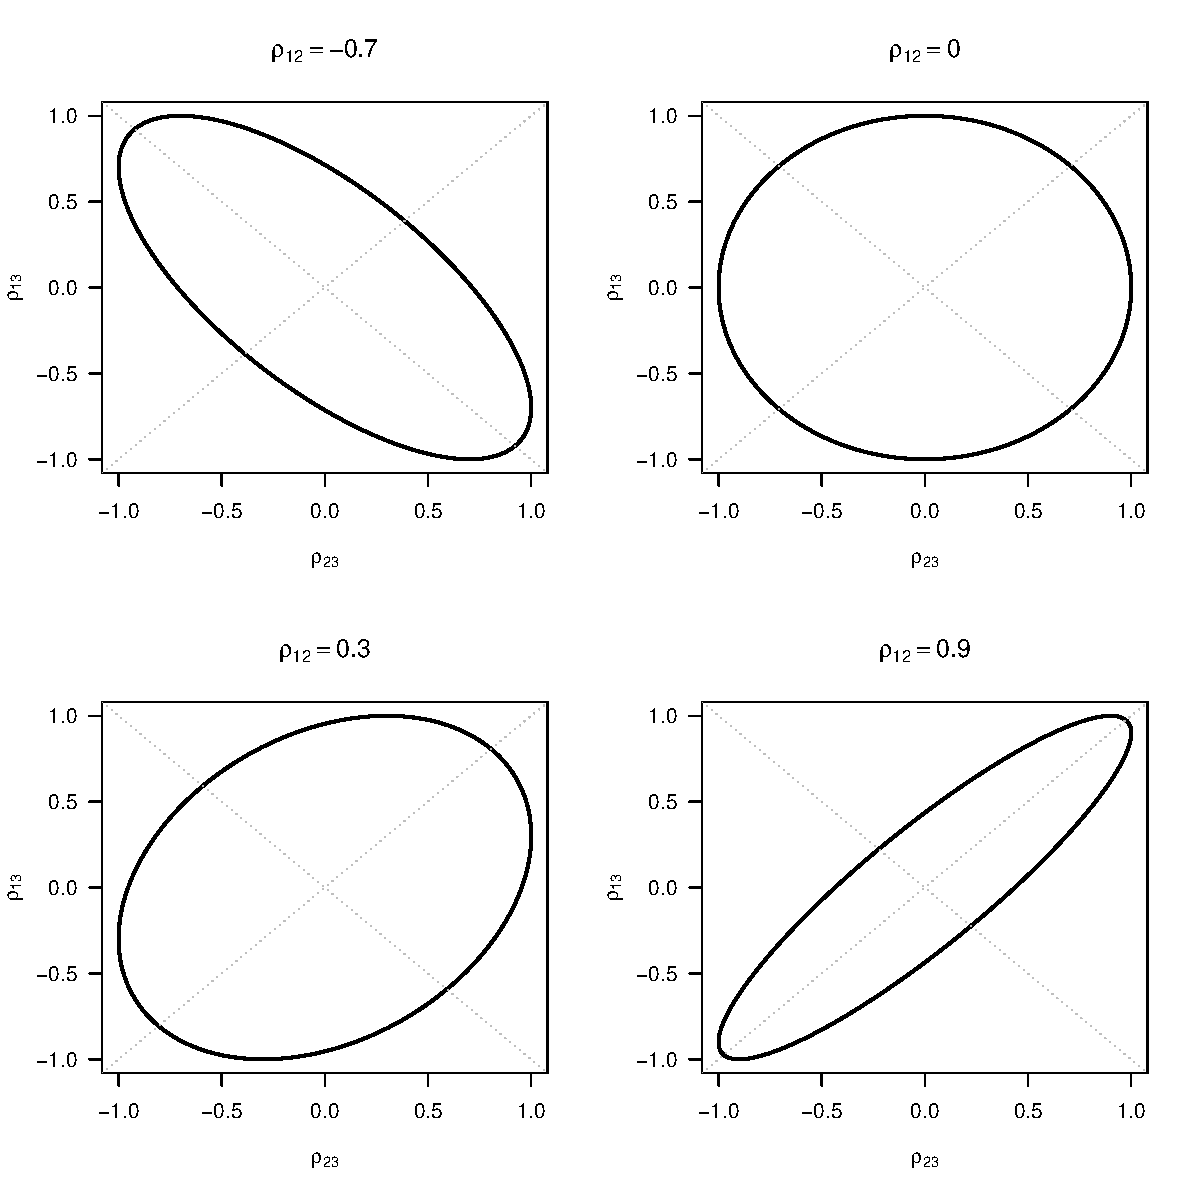
\includegraphics[scale=0.4]{figures/rho}
\par\end{centering}
\caption{The ellipses of Proposition \ref{prop:correlation identification}
for a selection of correlations $\rho_{12}$.}
\end{figure}
%
\begin{example}[{\textcite[p. 10]{Rassler2012-rp}}]
 Assume 
\[
\Phi=\left[\begin{array}{cc}
1 & 0.9 & \rho_{13}\\
0.9 & 1 & 0.8\\
\rho_{13} & 0.8 & 1
\end{array}\right].
\]
Applying Proposition \ref{prop:correlation identification} gives us
the identification set $(0.4585,0.9815)$ for $\rho_{13}$.
\end{example}


% \subsubsection{How many people know basic scientific facts?}
% \begin{quote}
% \textbf{\emph{Question 3}}: Does the Earth go around the Sun, or does
% the Sun go around the Earth?

% \medskip

% $\bigcirc$ Earth goes around the Sun.

% $\bigcirc$ Sun goes around the Earth.
% \end{quote}
% The National Science Board \citeyear[Table 7-8]{National_Science_Board2014-yl}
% reports that a shockingly high percentage of people answer this question incorrectly. Only $74$\% of American adults answered correctly, while an even worse $66$\% of adults in the European Union answered correctly. South Koreans did slightly better, at $86$\%. But the true percentage of Americans who know the Earth goes around the Sun is probably even lower than $74$\%. For a monkey would select either option with equal probability, and some humans probably do this too. The base-line of no knowledge is $50$\% correct answers, and we haven't corrected for this. So what's the real percentage of people of who knows that the Earth goes around the Sun? 

% A popular way to model people's state of knowledge is to use probability distributions. Imagine everyone has a probability distribution over the answers to Question 3. Denote this distribution $c$ and the proposition that the Earth goes around the Sun by $A$. Then the knowledge of a person is captured by $c(A)$, which encodes the probability of answering $A$. In philosophy, this is called a \emph{credence function} \parencite{Pettigrew2019-rk}.

% We want to know the percentage of people that knows the answer to $A$. Even if we knew everyone's credence function $c$, the answer to this question is not completely straightforward. Knowing or not knowing must involve a cutoff. For instance, you could claim that you know $A$ when you are at least $95\%$ certain of $A$ and $A$ is true. This cutoff is arbitrary, and could equally well have been $75\%$, $99\%$, or anything else. A natural restriction is to demand a certainty of more than $50\%$, but otherwise any percentage appears defensible. To take this arbitrariness of the cutoffs into account, let us say that a person $\alpha$-knows $A$ if $c(A)>\alpha$ and $A$ is true. Now we can restate the goal: we want to find the percentage of the population that $\alpha$-knows that the Earth orbits the sun.

% To model all of this, let $c$ be a credence function sampled according to $Q$ and $X\mid c$ sampled according to $c$,
% \[
% c\sim Q,\quad X\mid c\sim c.
% \]
% The next step is to decide on the possible space of distributions $Q$. \textcite[Chapter 2, endnote 28]{Caplan2018-oj} assumes that every person either knows $A$ with certainty or guesses with $50/50$ odds.
% In this case, $Q$ can be parametrized by $\gamma$, the proportion who knows for certain. Then $1-\gamma=2(1-P(A))$, hence $\gamma=1-2(1-P(A))=2(A)-1$. When $P(A)=0.74$ we get $\gamma=0.48$, hence just below $50\%$ of the population $\alpha$-knows the Earth goes around the Sun when $\alpha\geq0.5$. 

% But the assumption that every person either knows $A$ with certainty or guesses with $50/50$ odds does not look quite right. For why would there be no one who are, say, $90\%$ certain that the Sun goes around the Earth?

% In the spirit of \textcite{Manski2003-aq}, we will make no assumption about $Q$. Let $H_\alpha(\beta)$ be the identification region for $\alpha$-knowledge of Question 3 when $P(A) = \beta$. Then we get the following proposition.
% \begin{proposition}
% \label{prop:guessing regions}Let $P(A)=\beta\in(0,1)$. Then 
% \[
% H_{\alpha}(\beta)=\begin{cases}
% [(\beta-\alpha)/(1-\alpha),1], & \textrm{when }\beta>\alpha,\\
% (0,1), & \textrm{when }\beta=\alpha,\\{}
% [0,\beta/\alpha], & \textrm{when }\beta<\alpha.
% \end{cases}
% \]
% \end{proposition}

% \begin{proof}
% Assume $\beta>\alpha$. Let $B$ be the event that $c(A)\leq\alpha$
% and $C$ the event that $c(A)>\alpha$. Denote $P(A\mid B)=\alpha-\epsilon$,
% where $\epsilon\in[0,\alpha]$, assume $P(A\mid C)=\beta+\delta$,
% $\delta\in[0,1-\beta]$, and denote $P(C)=q$. By the law of total
% probability,
% \[
% P(A)=P(C)(\beta+\delta)+P(B)(\alpha-\epsilon).
% \]
% Since $\beta=P(A)$, $P(C)=q$, and $P(B)=1-q$, we get $\beta=q(\beta+\delta)+(1-q)(\alpha-\epsilon).$
% Rearrange to get $q=(\beta-\alpha+\epsilon)/(\beta-\alpha+\epsilon+\delta)$.
% This is maximized when $\delta=0$, when $q=1$. It is minimized when
% $\epsilon=0$ and $\delta=1-\beta$, when $q=(\beta-\alpha)/(1-\alpha).$

% That $H_\alpha(\beta)=(0,\beta/\alpha]$ when $\alpha\geq\beta$ can be verified by duality. For now $1-\alpha\leq 1-\beta$, and we can use the same analysis as above when regarding $A^c$ as the right answer. Hence the maximum is $1$ and the minimum is $(1-\beta-(1-\alpha))/(1-(1-\alpha)=(\alpha-\beta)/\alpha$. Turn back to the case when $A$ is the right by forming $1-(0,(\alpha-\beta)/\alpha)=(0,\beta/\alpha].$
% \end{proof}
% \begin{figure}
% \noindent \begin{centering}
% 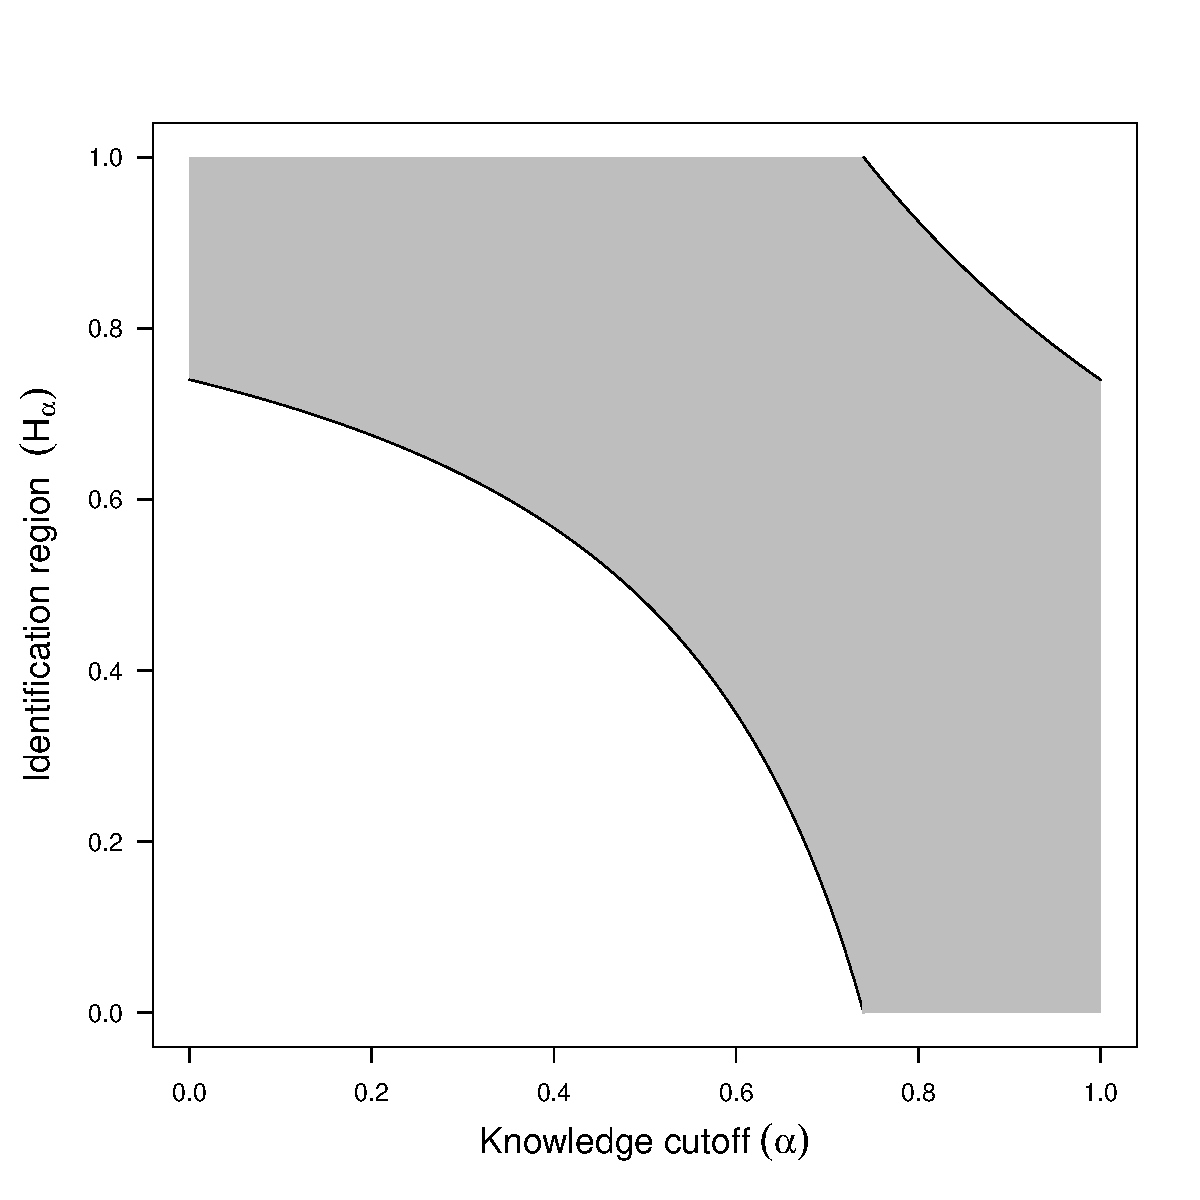
\includegraphics[scale=0.5]{figures/knowing}
% \par\end{centering}
% \caption{\label{fig:Identification-regions-guessing}Identification regions
% when $P(A)=0.74$.}
% \end{figure}

% The identification regions of Proposition \ref{prop:guessing regions} are wide. Figure \ref{fig:Identification-regions-guessing} tells the story when $\beta = P(A)=0.74$. In particular, when $\alpha=0.95$, we get $H_\alpha(\beta)=[0,0.78]$, meaning anything between $0\%$ and $78\%$ of the population knows $A$ with minimum $95\%$ certainty. If we choose the low $\alpha=0.6$, we get $H_\alpha(\beta)=[0.35,1]$, so at least $35\%$ of the population knows $A$ with minimum $60\%$ percent certainty. In conclusion, we can't really say how many Americans know that the Earth orbits the Sun.

\subsection{Identification of structural parameters}

Structural parameters are extra-probabilistical; they encode something
about the world that is not captured in any probability distribution.
Causal inference is about structural parameters; the joint distribution
of $(X,Y)$ does not tell us if $X$ causes $Y$. The causal information
is encoded in e.g. a causal graph \parencite{Pearl2009-zf} or a system
of counterfactuals \parencite[Chapter 4]{Pearl2016-tc}. A related example
of identification of structural parameters is from psychometrics.
In general, several structural equation models can give rise to exactly
the same joint distribution, but with highly disparate interpretations
\parencite{Raykov2001-ap}. Econometrics have perhaps the most famous
identification problem, sometimes called \textit{the identification problem in econometrics} \parencite{Manski1999-ab}.
\begin{example}[The identification problem in econometrics]
 Let $p$ be the price and $q$ the quantity of some good. Assume
the linear supply and demand functions
\begin{eqnarray*}
s(p) & = & \alpha_{s}+\beta_{s}p+\epsilon_{s}\quad\textrm{(supply)},\\
d(p) & = & \alpha_{d}+\beta_{d}p+\epsilon_{d}\quad\textrm{(demand).}
\end{eqnarray*}
Here $s(p)$ is the quantity supplied at the price $p$, $d(p)$ is
the quantity demanded at the price $p$, and $\epsilon_{1},\epsilon_{2}$
are uncorrelated error terms with zero mean and variances $\sigma_{1}^{2},\sigma_{2}^{2}$.
If prices are in equilibrium, $q=s(p)=d(p)$, hence
\[
q=\alpha_{s}+\beta_{s}p+\epsilon_{1}=\alpha_{d}+\beta_{d}p+\epsilon_{2}.
\]
We want to know the supply and demand functions, or equivalently,
$(\alpha_{s},\beta_{s},\alpha_{d},\beta_{d})$. We know the mean $\mu$
and covariance $\Sigma$ of $(p,q)$:
\begin{eqnarray*}
\mu & = & \left(\frac{\alpha_{d}-\alpha_{s}}{\beta_{s}-\beta_{d}},\frac{\beta_{s}\alpha_{d}-\beta_{d}\alpha_{s}}{\beta_{s}-\beta_{d}}\right)\\
\Sigma & = & \frac{1}{(\beta_{s}-\beta_{d})^{2}}\left[\begin{array}{cc}
\sigma_{1}^{2}+\sigma_{2}^{2} & \beta_{d}\sigma_{1}^{2}+\beta_{s}\sigma_{2}^{2}\\
\beta_{s}\sigma_{1}^{2}+\beta_{s}\sigma_{2}^{2} & \beta_{d}^{2}\sigma_{1}^{2}+\beta_{s}^{2}\sigma_{2}^{2}
\end{array}\right]
\end{eqnarray*}
Here we have $5$ knowns $(\mu_{1},\mu_{2},\Sigma_{11},\Sigma_{22},\Sigma_{12})$
and $6$ unknowns $$(\alpha_{s},\beta_{s},\alpha_{d},\beta_{d},\sigma_{1}^{2},\sigma_{2}^{2})$$
in a system of quadratic equations, which has no
unique solution. To rectify this, several identifying restrictions have been proposed. See \textcite[Chapter 6]{Manski1999-ab} for details.
\end{example}
    %\printbibliography[heading = subbibliography]

    \chapter{Paper summaries}
    \section{Please avoid the standardized alpha and the ordinal alpha}
\textbf{Moss, J. ``Please avoid the standardized alpha and the ordinal alpha''
(2020). Submitted for publication, \emph{Psychometrika.}}

The standardized alpha is a variant of coefficient alpha,
\begin{equation}
\hat{\alpha}=\frac{k}{k-1}\left(1-\frac{\tr{S}}{\boldsymbol{1}^{T}S\boldsymbol{1}}\right),\tag{\ref{eq:sample coefficient alpha}}
\end{equation}
based on the correlation matrix $R$ instead of the covariance matrix $S$. Assuming the one-factor linear model \eqref{eq:one-factor model}, the usage of standardized alpha can be justified in two ways. First, standardized alpha equals coefficient alpha under, the parallel model, which means that all loadings $\lambda_i$ are equal and all errors $\sigma_i$ are equal. Second, if one wishes to use the standardized sum-score, standardized alpha appears to be appropriate.

Neither of these justifications hold water. The conditions for standardized alpha to equal coefficient alpha are too stringent to be realistic, and there is no indication that standardized alpha performs better than coefficient even when they hold. Moreover, the standardized sum-scores are seldom if ever appropriate. The mean squared error-optimal weighted sum-scores outperform them, but so do other intuitive weightings. Finally, standardized alpha is just an approximation to the reliability when the sum-scores are used, and one can use plug-in estimators of the reliability with better performance.

Recall the normal-ogive model on page \pageref{eq:discretization model}, also called the discretized factor analysis model. The correlation matrix of the latent $X$ is called the polychoric correlation matrix whenever $X$ is normal. If we opt to use the normal-ogive model and want to provide a reliability estimate, it is natural to plug the estimated polychoric correlation matrix $\hat{\Phi}$ into the expression for coefficient alpha. \textcite{Zumbo2007-ap} calls the resulting reliability coefficient the ordinal alpha, and argues it should be preferred to the ordinary coefficient alpha. 

The reliability coefficient, can be interpreted as the prediction strength of $\hat{Z}$ as a predictor of $Z$. But under this interpretation, the ordinal alpha barely makes sense, as its natural associated predictor is based on the latent $X$, not $Z$. I argue against the ordinal alpha and suggest you use the $R^2$ based on the best predictor of $Z$ based on the observed variable $Y$, which is estimable when $X$ is normal.

\section{Partial identification of
latent correlations with binary data}
\textbf{Grønneberg, S., Moss, J., Foldnes, N. ``Partial identification of
latent correlations with binary data'' (2020). Invited to resubmit, major revision, \emph{Psychometrika.}}

The normal-ogive model \eqref{eq:discretization model} is popular and well-motivated, but has a major defect. As explained in section \ref{subsec:Normal-ogive models}, it is impossible to test if $X$ is multivariate normal. What's more, the assumption of normality is important, and violating can have serious consequences \parencite{Foldnes2019-ew}. 

Assume we know the distribution $p$ of $Y$, the discretized variable, which is binary. Without assuming that $X$ is multivariate normal, what can we say about latent correlation matrix, that is, the correlation of $X$? This turns out to a question of partial identifiability (p. \pageref{sec:partial identification}). We know $p$ but want to know latent $\rho(X)$.

It turns out we can say nothing about the latent correlation without imposing any restrictions on the distribution of $X$. In other words, the correlation matrix of $X$ is completely unidentified without assumptions on $X$; it can take on any value between $-1$ and $1$ for any distribution of $Y$. But it is possible to find non-trivial identification regions in some cases.

In particular, there are non-trivial identification regions when the marginals of $X$ are fixed and the copula is allowed to vary freely. Recall that a copula completely describes the dependence structure in multivariate $Y$; see e.g. \textcite{Nelsen2007-qj} for an introduction. The marginals affect the identification regions, but cannot be tested in a discretization model. Assuming normal marginals is common, and can be justified by appealing to the central limit theorem.

With binary data, the identification region for the latent correlation $\rho$ is a closed interval, with a simple formula when the marginals are uniform. When the marginals are uniform or normal, the resulting intervals are too wide to be of practical interest. 

This paper is the first step on the road towards understanding partial identification regions for discretization models of higher dimensionality and more than one cutoff, which is the setting where discretization models are usually used. Even though the results of this paper are negative, we will hopefully find more practical identification regions in more these settings.

\section{Modelling publication bias and \emph{p}-hacking}
\textbf{Moss, J., De Bin, R. ``Modelling publication bias and \emph{p}-hacking''
(2020), Invited to resubmit, major revision, \emph{Biometrics.}}

Publication bias is actually quite easy to model. Hedges' publication bias model \parencite{Hedges1992-ue} models \textit{p}-value based publication bias perfectly. But \textit{p}-hacking is much harder to deal with, partly as we do not have a solid understanding of how research \textit{p}-hack; partly as what we know is daunting to model efficiently. In this paper we explore a small modification of Hedges' publication bias model that turns it into a \textit{p}-hacking model instead. We argue the new model works well using examples, simulations, and theoretical arguments. 

The difference between Hedges' publication bias model and our \textit{p}-hacking model is subtle, and disappears if there is no heterogeneity in the data. In publication bias, a study is rejected with high probability if its \textit{p}-value is above $0.05$. In Hedges' model, a researcher whose study is rejected will attempt a completely new study -- and under heterogeneity, this study will have its own true effect size parameter $\theta_i$. In the \textit{p}-hacking model, a researcher will not attempt a new study if it fails to reach significance -- she will manipulate it until its \textit{p}-value is less than $0.05$. In this case, she will not deal with a new effect size $\theta_i$, but deal with the same all along.

This subtle modelling difference sometimes has large effects on the resulting effect size estimates $\theta_0$ and $\tau$. Moreover, the \textit{p}-hacking model appears to work just as well, if not better, on meta-analyses we strongly suspect have been subject to both \textit{p}-hacking and publication bias.

\section{Infinite confidence sets in Hedges' model of publication
bias}
\textbf{Moss, J. ``Infinite confidence sets in Hedges' model of publication
bias'' (2020). Submitted for publication, \emph{Austrian Journal of Statistics.}
}

Hedges' publication bias model is one of the most popular models of publication bias. Interpreting this model is a breeze, and it is evidently the correct model for \textit{p}-value based publication bias. But the model is not above reproach. Several authors have complained about difficulties with estimation and inference using maximum likelihood, with parameter estimates being all over the place and algorithms failing to converge. What causes these problems and how can we interpret them?

\textcite{Gleser1987-ii} proved an elegant theorem giving sufficient conditions for every confidence set to be of infinite diameter with positive probability. If we could show that a model's confidence sets must be of infinite diameter using this theorem, we would immediately be justified in comparing it to other models with such poorly-behaved confidence sets. And in this paper I show that every confidence set for Hedges' publication bias model is of infinite diameter, thereby giving an explanation for the model's unsavoury behavior.
    \printbibliography[heading = bibliography, title = References]
    
    \paper              
    \paperpage          
    \numberofpapers{4} 

    \documentclass{standalone}

% Standalone ensures that
% everything from \documentclass to \begin{document}
% in this document is ignored when included by main.tex.

\begin{document}

\author
{
    Jonas Moss
}
\title{Please avoid the standardized alpha and the ordinal alpha}
\metadata{Submitted for publication. PsyArXiv: \url{https://psyarxiv.com/nvg5d/}
}
\maketitle

\includearticle{papers/paperI.pdf}

\end{document}\clearpage
    \documentclass{standalone}

\begin{document}

\author
{
    Steffen Grønneberg \and
    Jonas Moss \and
    Njål Foldnes
}
\title{Partial identification of latent correlations with binary data}
\metadata{Invited to resubmit, major revision, \emph{Psychometrika}.}
\maketitle

\includearticle{papers/paperII.pdf}

\end{document}\clearpage
    \documentclass{standalone}

\begin{document}

\author
{
    Jonas Moss \and
    Riccardo De Bin
}
\title{Modelling publication bias and p-hacking}
\metadata{Invited to resubmit, major revision, \emph{Biometrics}. \arxiv{1911.12445}}
\maketitle

\includearticle{papers/paperIII.pdf}

\end{document}\clearpage
    \documentclass{standalone}

\begin{document}

\author
{
    Jonas Moss
}
\title{Infinite confidence sets in Hedges' model of publication
bias}
\metadata{Submitted for publication, \emph{Austrian Journal of Statistics}. \arxiv{1912.09180}}
\maketitle

\includearticle{papers/paperIV.pdf}

\end{document}\clearpage

    \swpaper              
    \swpaperpage          
    \numberofswpapers{2} 
    \documentclass{standalone}

\begin{document}

\author
{
    Jonas Moss \and Martin Tveten
}
\title{kdensity: An R package for kernel
density estimation with parametric starts and asymmetric kernels.}
\metadata{Published in \emph{Journal of Open Source Software}, 2019, \doi{10.21105/joss.01566}.}
\swmaketitle

\includearticle{swpapers/swpaperI.pdf}

\end{document}\clearpage
    \documentclass{standalone}

\begin{document}

\author
{
    Jonas Moss
}
\title{univariateML: An R package for maximum likelihood
estimation of univariate densities.}
\metadata{Published in \emph{Journal of Open Source Software}, 2019, \doi{10.21105/joss.01863}.}
\swmaketitle

\includearticle{papers/swpaperII.pdf}

\end{document}\clearpage
    
        
    \appendix           % "Chapter" is renamed "Appendix"
    \theappendixpage       % Similar to \part*{Appendices}, but appears in TOC
    \chapter{Supplementary Material for "Partial Identification of Latent Correlations with Binary Data"}
\section*{Description}

\begin{description}
\item[utility.R] Includes functions to compute the bounds from Proposition 1 with normal marginals, bounds from Proposition 2 (Spearman's rho), as well as Spearman's rho of Z when Z is known to have a normal copula.

\item[1.R] Gives basic illustrations of the functions in utility.R by reproduces the empirical examples from the paper.

\item[2.R] Simulates from the extremal distributions (and contains code to plot simulated data from the distributions). Verifies the numerical procedures in the "lcorr"-package via Monte Carlo integration.

\item[3.R] Verifies the numerical procedures in the "lcorr"-package via a brute force numerical integration method.

\item[4.R]  Contains code for the biserial example. Can be extended to other datasets.

\item[5.R]  Contains code for numerical exploration of the bounds as given in the two figures in the appendix.

\item[6.R]  Contains code for approximate the minimum length of the bounds.

\item[plot.R]  Code for the colorful plot in the appendix.
\end{description}
\section*{utility.R}
\lstinputlisting[language=R, breaklines=true, basicstyle=\small]{code/utility.R}
\section*{1.R}
\lstinputlisting[language=R, breaklines=true, basicstyle=\small]{code/1.R}
\section*{2.R}
\lstinputlisting[language=R, breaklines=true, basicstyle=\small]{code/2.R}
\section*{3.R}
\lstinputlisting[language=R, breaklines=true, basicstyle=\small]{code/3.R}
\section*{4.R}
\lstinputlisting[language=R, breaklines=true, basicstyle=\small]{code/4.R}
\section*{5.R}
\lstinputlisting[language=R, breaklines=true, basicstyle=\small]{code/5.R}
\section*{6.R}
\lstinputlisting[language=R, breaklines=true, basicstyle=\small]{code/6.R}
\section*{plot.R}
\lstinputlisting[language=R, breaklines=true, basicstyle=\small]{code/plot.R}

    \chapter{Supporting Information for "Modelling publication bias and \textit{p}-hacking"}

\section*{Web Appendix A}

Recall that a density $f(x;\theta)$ is identified if $f(x;\theta_{1})=f(x;\theta_{2})$
for all $x$ implies that $\theta_{1}=\theta_{2}.$ Call a density
$f(x;\theta)$ \textit{strongly identified} if $f(x;\theta_{1})/f(x;\theta_{2})$
being constant for all $x$ in an open interval $I$ implies that
$\theta_{1}=\theta_{2}$.
\paragraph{Proposition A.}\label{prop:identified}

Let $f(x;\theta)$ be a family of densities on $\mathbb{R}$, $-\infty=a_{1}<a_{2}<\ldots<a_{k+1}=\infty$
a sequence of cutoffs, and $f_{[a_{i},a_{i+1}]}(x;\theta)$ the density
$f$ truncated to $[a_{i},a_{i+1}]$. Let $\lambda_{i},k=1,\ldots k$
be positive numbers satisfying $\sum_{i=1}^{k}\lambda_{i}=1$. Then
the mixture
\[
g(x;\lambda,\theta)=\sum_{i=1}^{k}\lambda_{i}f_{[a_{i},a_{i+1})}(x;\theta)
\]
is identified in $(\lambda,\theta)$ if $f(x;\theta)$ is strongly
identified in $\theta$.

\paragraph{Proof.}
Assume that $g(x;\lambda_{1},\theta_{1})=g(x;\lambda_{2},\theta_{2})$.
Then $$\lambda_{1i}f_{[a_{i},a_{i+1}]}(x;\theta_{1})=\lambda_{2i}f_{[a_{i},a_{i+1}]}(x;\theta_{2})$$
for all $i$, thus
\[
\frac{\lambda_{1i}}{\lambda_{2i}}=\frac{f_{[a_{i},a_{i+1})}(x;\theta_{1})}{f_{[a_{i},a_{i+1})}(x;\theta_{2})}.
\]
This implies that $f(x;\theta_{1})/f(x;\theta_{2})$ is constant for
$x\in[a_{i},a_{i+1}]$. But since $f(x;\theta)$ is strongly identifiable,
$\theta_{1}=\theta_{2}$, and, consequently, $\lambda_1 = \lambda_2$.


If $f(x;\theta)$ is real analytic and nowhere zero, $f(x;\theta_{1})/f(x;\theta_{2})$
is also real analytic and nowhere zero. By the Identity Theorem \parencite[Corollary 1.2.6]{Krantz2002-bt}, if the ratio
$f(x;\theta_{1})/f(x;\theta_{2})$ is constant on some interval $I$,
then $f(x;\theta_{1})/f(x;\theta_{2})$ is constant everywhere, hence
$f(x;\theta_{1})=f(x;\theta_{2})$ everywhere. Thus a family of real
analytic nowhere zero densities is identified if and only if it is
strongly identified. Every exponential family of densities on the form
\[
f(x;\theta)=h(x)\exp(\eta(\theta)^{T}T(x)-A(\theta))
\]
satisfies this property, provided only that $h$ is nowhere zero real analytic
and $T$ is real analytic. In particular, the normal family satisfies
the properties.

Not every density is strongly identified. For instance, mixtures of uniforms are not strongly identified. And indeed, Proposition A fails when $f$ is a mixture of uniforms.

\section*{Web Appendix B}

As mentioned in Section 2, any \textit{p}-hacking model can be written on the form of a selection model. Observe that
\begin{eqnarray*}
\int_{[0,1]}f_\alpha^{\star}(x_{i}\mid\theta_{i},\eta_{i}, u)d\omega(\alpha) & = & \int_{[0,1]}f(x_{i}\mid\theta_{i})P(u\in\left[0,\alpha\right]\mid\theta_{i},\eta_{i})^{-1}d\omega(\alpha)\\
 & = & f(x_{i}\mid\theta_{i})\int_{[0,u]}P(u\in\left[0,\alpha\right]\mid\theta_{i},\eta_{i})^{-1}d\omega(\alpha).
\end{eqnarray*}
where $f_\alpha^{\star}$ is the density $f^{\star}$ truncated so that the \textit{p}-value $u\in\left[0,\alpha\right]$. This is a publication bias model if $$h(u)=\int_{[0,u]}P(u\in\left[0,\alpha\right]\mid\theta_{i},\eta_{i})^{-1}d\omega(\alpha)$$ is bounded for each $u$ and $h(u)$ is independent of $\theta_{i},\eta_{i}$. While $h(u)$ can be bounded, it is typically dependent of $\theta_{i},\eta_{i}$, with the fixed effect model under complete selection for significance being a notable exception.

On the other hand, any selection model $f(x_{i};\theta_{i},\eta_{i})\rho(u)$ with $I =\int f(x;\theta_{i},\eta_{i})\rho(u)du<\infty$ can be written as a mixture model. For then there is a finite measure $d\omega(\alpha;\theta_{i},\eta_{i})$ satisfying 
\[
\rho(u)=\int_{[0,u]}\frac{1}{P(u\in\left[0,\alpha\right]\mid\theta,\eta)}d\omega(\alpha;\theta_{i},\eta_{i})
\]
Just take $d\omega(\alpha;\theta_{i},\eta_{i})=d\rho(\alpha)P(u\in\left[0,\alpha\right]\mid\theta_{i},\eta_{i})$, where $d\rho(\alpha)$ is defined by $\int_{0}^{u}d\rho(\alpha)=\rho(u)$. The size of the measure is
\begin{eqnarray*}
\int_{0}^{1}d\omega(\alpha;\theta_{i},\eta_{i}) & = & \int_{0}^{1}P(u\in\left[0,\alpha\right]\mid\theta_{i},\eta_{i})d\rho(\alpha)\\
 & = & \int_{0}^{1}f(u;\theta_{i},\eta_{i})\int_{0}^{u}d\rho(\alpha)du\\
 & = & I
\end{eqnarray*}
Hence $I_{\theta,\eta}d\omega'(\alpha;\theta_{i},\eta_{i})$ is a probability measure. This probability measure makes 
\[
I^{-1}f(x_{i};\theta_{i},\eta_{i})\rho(u)=\int_{[0,1]}f_\alpha(x_{i};\theta_{i},\eta_{i})d\omega'(\alpha)
\]
as can be seen by the following computation,
\begin{eqnarray*}
I^{-1}f(x_{i};\theta_{i},\eta_{i})\rho(u) & = & I^{-1}\int_{[0,u]}\frac{f(x_{i};\theta_{i},\eta_{i})}{P(u\in\left[0,\alpha\right]\mid\theta_{i},\eta_{i})}d\omega(\alpha)\\
 & = & I^{-1}\int_{[0,1]}\frac{f(x_{i};\theta,\eta)1_{\left[0,\alpha\right]}(u)}{P(u\in\left[0,\alpha\right]\mid\theta_{i},\eta_{i})}d\omega(\alpha)\\
 & = & I^{-1}\int_{[0,1]}f_\alpha(x_{i};\theta_{i},\eta_{i})d\omega(\alpha)\\
 & = & \int_{[0,1]}f_\alpha(x;\theta_{i},\eta_{i})d\omega'(\alpha)
\end{eqnarray*}

Proposition 1 shows the form of the one-sided normal step function selection probability publication bias model when it is written as a mixture model of the form (5). But most such mixture models are not true \textit{p}-hacking models, as the mixing probabilities $\pi_{i}^{\star}$ depend on $\theta$. There is no way for the \textit{p}-hacker to know
$\theta$, so we cannot regard the publication bias model as a \textit{p}-hacking model.


    


\end{document}